\chapter{无稳定化项虚单元方法}
本章节给出一种无稳定化项的虚单元方法,
假设多面体单元 $K$ 被剖分为一个单纯形网格 $\mathcal T_K$。
我们在 $\mathcal{T}_K$ 上定义一个 $H(\diver)$ 协调的宏有限元空间,
其满足在边界上法向分量以及散度值是多项式,
从而可以计算虚单元函数梯度到这个空间的 $L^2$ 投影 $Q_k^{\diver}$。
我们建立了 $H(\diver)$ 协调的宏有限元空间上的一个范数等价性,
基于此我们提出了二阶椭圆方程的无稳定化项 
$H^1$ 协调、非协调虚单元方法,证明了 $Q_k^{\diver}$ 投影前后的函数的范数等价性,
给出了方法的稳定性,
收敛性,最后通过大量数值算例验证了收敛性,并与标准方法做出对比。

\section{网格假设}
本章节要求网格 $\mathcal T_h$ 满足以下假设条件:
\begin{itemize}
    \item[(A1)] 对于任意单元 $K\in \mathcal T_h$, $F\in \mathcal F_h^r$ ($1\leq
        r\leq d-1$),都是星形的,具有一致有界的 chunkiness 参数。

 \item[(A2)] 存在一个形状正则的单纯形网格 $\mathcal T_h^*$,使得每个 $K\in
     \mathcal T_h$ 都是 $\mathcal T_h^*$ 中某些单纯形的并集。对于多面体 $K\in
     \mathcal T_h$,令 $\mathcal T_K$ 表示从 $\mathcal T_h^*$ 导出的 $K$
     的单纯形分割。假设单纯形分割 $\mathcal T_K$ 是拟一致的。
\end{itemize}
在本章节中,我们使用“$\lesssim\cdots $”表示“$\leq C\cdots$”,其中 $C$
是一个与网格尺寸 $h$
无关的通用正常常数,但可能依赖于多面体的 chunkiness 参数、多项式的次数 $k$、空间维数
$d$,以及虚拟三角剖分 $\mathcal T^*_h$
的形状正则性和准均匀常数,这些常数在不同情况下可能取不同的值。记 $A\eqsim B$
表示 $A\lesssim B$ 且 $B\lesssim A$。

设 $\mathcal{F}(\mathcal{T}_K)$ 和 $\mathcal{E}(\mathcal{T}_K)$ 分别表示单纯形剖分 $\mathcal{T}_K$ 中所有 $(d-1)$ 维面与 $(d-2)$ 维面的集合。定义  
\[
\mathcal{F}^{\partial}(\mathcal{T}_K):=\{F\in\mathcal{F}(\mathcal{T}_K): F\subset\partial K\},\quad \mathcal{E}^{\partial}(\mathcal{T}_K):=\{e\in\mathcal{E}(\mathcal{T}_K): e\subset\partial K\}.
\]
在本章节中,我们使用 $T$ 表示一个单纯形,使用 $K$ 表示一个一般的多面体。
\section{$H(\diver)$-协调的宏有限元}
在这一部分,我们将构造任意维 $H(\diver)$-协调的宏有限元空间
$\mathbb{V}_{k-1}^{\rm div}(K)$ 及相应的自由度,建立
$\boldsymbol{\phi}\in\mathbb{V}_{k-1}^{\rm div}(K)$ 的 $L^2$ 范数等价关系
\begin{equation*}%\label{eq:Vkm1divnormequiv}
\|\boldsymbol{\phi}\|_{0,K}\eqsim h_K\|\diver\boldsymbol{\phi}\|_{0,K} + \sup_{\boldsymbol{\psi}\in\diver\mathring{\boldsymbol{V}}_{k}^{d-2}(K)}\frac{(\boldsymbol{\phi}, \boldsymbol{\psi})_K}{\|\boldsymbol{\psi}\|_{0,K}} +\sum_{F\in\mathcal F(K)}h_F^{1/2}\|\boldsymbol{\phi}\cdot\boldsymbol{n}\|_{0,F}.
\end{equation*}
空间 $\mathbb{V}_{k-1}^{\rm div}(K)$ 及其 $L^2$ 范数等价性将用于证明虚单元空间的范数等价性
\begin{equation*}%\label{intro:gradVknormequiv}
\|Q_{K,k-1}^{\diver}\nabla v\|_{0,K}\eqsim \|\nabla v\|_{0,K} \quad \forall~v\in V_k(K),
\end{equation*}
其中 $V_k(K)$ 是第 \ref{sec:stabfreencfmvem} 节中的非协调虚单元空间或第
\ref{sec:stabfreecfmvem} 节中的协调虚单元空间。这里 $Q_{K,k-1}^{\diver}$
是到空间 $\mathbb{V}_{k-1}^{\rm div}(K)$ 上的 $L^2$ 投影。

\subsection{$H(\diver)$-协调的有限元}
对于 $d$ 维多面体 $K\in \mathcal T_h$ 和 $k\geq2$,定义
\[
\boldsymbol{V}_{k-1}^{\mathrm{BDM}}(K):=\{\boldsymbol{\phi}\in\boldsymbol{H}(\diver,
K): \boldsymbol{\phi}|_{T}\in \mathbb P_{k-1}(T;\mathbb R^d) \forall
T\in\mathcal T_K\}.
\]
为局部的 BDM 元空间~\cite{BrezziDouglasMarini1986,BrezziDouglasDuranFortin1987,Nedelec:1986family},其自由度由 \cite{ChenHuang2021divdiv} 给出
\begin{align}
(\boldsymbol{v}\cdot\boldsymbol{n}, q)_F, & \quad q\in \mathbb P_{k-1}(F), F\in\mathcal F(T), \label{BDMdof1} \\
(\diver\boldsymbol{v}, q)_T, & \quad q\in \mathbb P_{k-2}(T)/\mathbb R, \label{BDMdof2} \\
(\boldsymbol{v}, \boldsymbol{q})_T, & \quad \boldsymbol{q}\in \mathbb
P_{k-3}(T;\mathbb K)\boldsymbol{x} \label{BDMdof3}.
\end{align}
对于 $T\in\mathcal T_K$。这里 $\mathbb P_{k-2}(T)/\mathbb R:=\mathbb P_{k-2}(T)\cap L_0^2(T)$,$\mathbb P_{k-3}(T;\mathbb K)\boldsymbol{x}:=\{\boldsymbol{\tau}\boldsymbol{x}: \boldsymbol{\tau}\in \mathbb P_{k-3}(T;\mathbb K)\}$,$\boldsymbol{x}\in T$ 是独立变量。
定义 $\mathring{\boldsymbol{V}}_{k-1}^{\mathrm{BDM}}(K):=\boldsymbol{V}_{k-1}^{\mathrm{BDM}}(K)\cap \boldsymbol{H}_0(\diver, K)$。

对于最低阶情况我们定义 RT 元空间~\cite{RaviartThomas1977,Nedelec1980}
\[
\boldsymbol{V}^{\mathrm{RT}}(K):=\{\boldsymbol{\phi}\in\boldsymbol{H}(\diver,
    K): \boldsymbol{\phi}|_{T}\in \mathbb P_{0}(T;\mathbb
R^d)+\boldsymbol{x}\mathbb P_{0}(T) \forall T\in\mathcal T_K\}.
\]
其自由度为
\[
(\boldsymbol{v}\cdot\boldsymbol{n}, q)_F,  \quad q\in \mathbb P_{0}(F), F\in\mathcal F(T)
, T\in\mathcal T_K.
\]
定义 $\mathring{\boldsymbol{V}}^{\mathrm{RT}}(K):=\boldsymbol{V}^{\mathrm{RT}}(K)\cap \boldsymbol{H}_0(\diver, K)$。

\subsection{有限元微分 $(d-2)$-形式}
重申 \cite{ArnoldFalkWinther2006, Arnold2018} 中的有限元微分
$(d-2)$-形式,即 $H\Lambda^{d-2}$-协调有限元。
我们将使用微分形式的矩阵、向量代理来展示有限元微分 
$(d-2)$-形式。

由 \cite{ChenHuang2021divdiv} 中的 (3.5) 式,我们有如下直和分解:
\begin{equation}\label{eq:Pkvectordecomp}
\mathbb P_{k-1}(T;\mathbb R^{d})=\nabla\mathbb P_k(T)\oplus\mathbb P_{k-2}(T;\mathbb K)\boldsymbol{x}.
\end{equation}
% {其中 $\mathbb P_{k-2}(T;\mathbb K)\boldsymbol{x}:=\{\boldsymbol{\tau}\boldsymbol{x}: \boldsymbol{\tau}\in \mathbb P_{k-2}(T;\mathbb K)\}$,其中 $\boldsymbol{x}\in T$ 是自变量。}
回顾 \cite[(35)]{Chen;Huang:2020Finite},我们有
\begin{equation}\label{eq:20230205}
\mathbb P_{k}(T)\cap\ker(I+\boldsymbol{x}\cdot\nabla)=\{0\}.
\end{equation}

\begin{lemma}\label{lem:mathrm{skw}grad}
对于 $\boldsymbol{w}\in\mathbb P_{k-2}(T;\mathbb K)\boldsymbol{x}$,满足 $(\mathrm{skw}\nabla\boldsymbol{w})\boldsymbol{x}=\boldsymbol{0}$,则 $\boldsymbol{w}=\boldsymbol{0}$。
\end{lemma}
\begin{proof}
由于
\begin{equation*}%\label{eq:20220224}  
(\mathrm{skw}\nabla\boldsymbol{w})\boldsymbol{x}=\frac{1}{2}(\nabla\boldsymbol{w})\boldsymbol{x}-\frac{1}{2}(\nabla\boldsymbol{w})^{\intercal}\boldsymbol{x}=\frac{1}{2}\nabla(\boldsymbol{w}\cdot\boldsymbol{x})-\frac{1}{2}(I+\boldsymbol{x}\cdot\nabla)\boldsymbol{w},
\end{equation*}
我们得到 $\boldsymbol{w}\cdot\boldsymbol{x}=0$,从而 $(I+\boldsymbol{x}\cdot\nabla)\boldsymbol{w}=\boldsymbol{0}$,这与 \eqref{eq:20230205} 结合可以得出 $\boldsymbol{w}=\boldsymbol{0}$。
\end{proof}

\begin{lemma}
多项式复形
\begin{equation}\label{eq:polycomplex1}
\mathbb R\xrightarrow{}\mathbb P_k(T)\xrightarrow{\nabla}\mathbb
P_{k-1}(T;\mathbb R^d)\xrightarrow{\mathrm{skw}\nabla}\mathbb P_{k-2}(T;\mathbb
K).
\end{equation}
是恰当的。
\end{lemma}
\begin{proof}
显然 \eqref{eq:polycomplex1} 是一个复形。我们只需证明 $\mathbb P_{k-1}(T;\mathbb R^d)\cap\ker(\mathrm{skw}\nabla)\subseteq\nabla\mathbb P_{k}(T)$。

对于 $\boldsymbol{v}\in\mathbb P_{k-1}(T;\mathbb R^d)\cap\ker(\mathrm{skw}\nabla)$,根据分解 \eqref{eq:Pkvectordecomp},存在 $q\in \mathbb P_k(T)$ 和 $\boldsymbol{w}\in\mathbb P_{k-2}(T;\mathbb K)\boldsymbol{x}$ 使得 $\boldsymbol{v}=\nabla q+\boldsymbol{w}$。通过 $\mathrm{skw}\nabla\boldsymbol{v}=\boldsymbol{0}$,我们得到 $\mathrm{skw}\nabla\boldsymbol{w}=\boldsymbol{0}$。应用引理~\ref{lem:mathrm{skw}grad} 可得 $\boldsymbol{w}=\boldsymbol{0}$。因此,$\boldsymbol{v}=\nabla q\in\nabla\mathbb P_k(T)$。
\end{proof}

\begin{lemma}  
存在如下分解:
\begin{equation}\label{eq:Pkskwtensordecomp}  
\mathbb P_{k-2}(T;\mathbb K)=\skw\nabla\mathbb P_{k-1}(T;\mathbb R^d)\oplus\big(\mathbb P_{k-2}(T;\mathbb K)\cap\ker(\boldsymbol{x})\big),
\end{equation}  
其中
$
\mathbb P_{k-2}(T;\mathbb K)\cap\ker(\boldsymbol{x}):=\{\boldsymbol{\tau}\in\mathbb P_{k-2}(T;\mathbb K): \boldsymbol{\tau}\boldsymbol{x}=\boldsymbol{0}\}.
$
\end{lemma}  
\begin{proof}  
根据分解 \eqref{eq:Pkvectordecomp},我们有
\[
\mathrm{skw}\nabla\mathbb P_{k-1}(T;\mathbb R^d)=\mathrm{skw}\nabla(\mathbb P_{k-2}(T;\mathbb K)\boldsymbol{x}).
\]
通过引理~\ref{lem:mathrm{skw}grad},$\mathrm{skw}\nabla\mathbb P_{k-1}(T;\mathbb
R^d)\cap\big(\mathbb P_{k-2}(T;\mathbb
K)\cap\ker(\boldsymbol{x})\big)=\{\boldsymbol{0}\}$。所以我们只需检查维数。
根据复形 \eqref{eq:polycomplex1}的恰当性可知
\begin{equation}\label{eq:20220324-1}
\dime\mathrm{skw}\nabla\mathbb P_{k-1}(T;\mathbb R^d)=\dime\mathbb P_{k-1}(T;\mathbb R^d)-\dime\nabla\mathbb P_k(T).
\end{equation}
另一方面,通过空间分解 \eqref{eq:Pkvectordecomp},
\[
\dime\mathbb P_{k-2}(T;\mathbb K)\boldsymbol{x}=\dime\mathbb P_{k-1}(T;\mathbb R^{d})-\dime\nabla\mathbb P_k(T).
\]
因此,$\dime\mathrm{skw}\nabla\mathbb P_{k-1}(T;\mathbb R^d)=\dime\mathbb
P_{k-2}(T;\mathbb K)\boldsymbol{x}$,这证明了分解
\eqref{eq:Pkskwtensordecomp}。
\end{proof}

由 \eqref{eq:Pkskwtensordecomp} 和 \eqref{eq:20220324-1},我们得到
\begin{equation}\label{eq:20220324-2}
\dime\mathbb P_{k-2}(T;\mathbb K)\cap\ker(\boldsymbol{x})=\dime\mathbb P_{k-2}(T;\mathbb K)+\dime\nabla\mathbb P_k(T)- \dime\mathbb P_{k-1}(T;\mathbb R^d).
\end{equation}

有了分解 \eqref{eq:Pkskwtensordecomp} 和 $\mathbb{P}_{k-1}(F;\mathbb
R^{d-1})=\nabla_F \mathbb{P}_k(F)\oplus\mathbb P_{k-2}(F;\mathbb
K)\boldsymbol{x}$,我们可以定义微分$(d-2)$-形式的有限元。将 $\mathbb
P_k(T;\mathbb K)$ 作为形函数的空间。其自由度由以下给出:
\begin{align}
((\boldsymbol{n}_1^e)^{\intercal}\boldsymbol{\tau}\boldsymbol{n}_2^e, q)_e, & \quad q\in \mathbb P_k(e), e\in\mathcal E(T), \label{eq:-2formfemdof1} \\
(\diver_F(\boldsymbol{\tau}\boldsymbol{n}), q)_F, & \quad q\in \mathbb P_{k-1}(F)/\mathbb R, F\in\mathcal F(T), \label{eq:-2formfemdof21} \\
(\boldsymbol{\tau}\boldsymbol{n}, \boldsymbol{q})_F, & \quad \boldsymbol{q}\in \mathbb P_{k-2}(F;\mathbb K)\boldsymbol{x}, F\in\mathcal F(T), \label{eq:-2formfemdof22} \\
(\diver\boldsymbol{\tau}, \boldsymbol{q})_T, & \quad \boldsymbol{q}\in\mathbb P_{k-3}(T;\mathbb K)\boldsymbol{x}, \label{eq:-2formfemdof31} \\
(\boldsymbol{\tau}, \boldsymbol{q})_T, & \quad \boldsymbol{q}\in \mathbb P_{k-2}(T;\mathbb K)\cap\ker(\boldsymbol{x}). \label{eq:-2formfemdof32}
\end{align}
在自由度 \eqref{eq:-2formfemdof1} 中,$\boldsymbol{n}_1^e$ 和  $\boldsymbol{n}_2^e$ 是 $e$ 的两个单位法向量,满足 $\boldsymbol{n}_1^e\cdot\boldsymbol{n}_2^e=0$。

\begin{lemma}\label{lem:normalskwtensor}
对于 $e\in\mathcal E(T)$,设 $\tilde{\boldsymbol{n}}_1$ 和  $\tilde{\boldsymbol{n}}_2$ 是另外两个单位法向量,满足 $\tilde{\boldsymbol{n}}_1\cdot\tilde{\boldsymbol{n}}_2=0$。那么
\[
\mathrm{skw}(\tilde{\boldsymbol{n}}_1\tilde{\boldsymbol{n}}_2^{\intercal})=\pm\mathrm{skw}(\boldsymbol{n}_1^e(\boldsymbol{n}_2^e)^{\intercal}).
\]
\end{lemma}

\begin{proof}
存在一个正交矩阵 $H\in\mathbb R^{2\times2}$,使得 $(\tilde{\boldsymbol{n}}_1,
\tilde{\boldsymbol{n}}_2)=(\boldsymbol{n}_1^e, \boldsymbol{n}_2^e)H$,
那么
\begin{align*}
2\mathrm{skw}(\tilde{\boldsymbol{n}}_1\tilde{\boldsymbol{n}}_2^{\intercal})&=\tilde{\boldsymbol{n}}_1\tilde{\boldsymbol{n}}_2^{\intercal}-\tilde{\boldsymbol{n}}_2\tilde{\boldsymbol{n}}_1^{\intercal}=(\tilde{\boldsymbol{n}}_1, \tilde{\boldsymbol{n}}_2)\begin{pmatrix}
0 & 1 \\
-1 & 0
\end{pmatrix}\begin{pmatrix}
\tilde{\boldsymbol{n}}_1^{\intercal} \\
\tilde{\boldsymbol{n}}_2^{\intercal}
\end{pmatrix}
\\
&=(\boldsymbol{n}_1^e, \boldsymbol{n}_2^e)H\begin{pmatrix}
0 & 1 \\
-1 & 0
\end{pmatrix}H^{\intercal}(\boldsymbol{n}_1^e, \boldsymbol{n}_2^e)^{\intercal}.
\end{align*}
显然 $H\begin{pmatrix}
0 & 1 \\
-1 & 0
\end{pmatrix}H^{\intercal}={\rm det}(H)\begin{pmatrix}
0 & 1 \\
-1 & 0
\end{pmatrix}$,因此
$
2\mathrm{skw}(\tilde{\boldsymbol{n}}_1\tilde{\boldsymbol{n}}_2^{\intercal})=2{\rm det}(H)\mathrm{skw}(\boldsymbol{n}_1^e(\boldsymbol{n}_2^e)^{\intercal}),
$
结论得证。
\end{proof}

\begin{lemma}\label{lem:-2formfemfaceunisolvence}
设 $\boldsymbol{\tau}\in\mathbb P_k(T;\mathbb K)$,$F\in\mathcal F(T)$。
假设 \eqref{eq:-2formfemdof1}-\eqref{eq:-2formfemdof22} 在 $F$ 上的自由度都为零。那么 $\boldsymbol{\tau}\boldsymbol{n}|_F=\boldsymbol{0}$。
\end{lemma}
\begin{proof}
由于 \eqref{eq:-2formfemdof1}可知:对于任意 $e\in\mathcal E(F)$,
$(\boldsymbol{n}_1^e)^{\intercal}\boldsymbol{\tau}\boldsymbol{n}_2^e|_e=0$,
结合引理~\ref{lem:normalskwtensor}
可得
$\boldsymbol{n}_{F,e}^{\intercal}\boldsymbol{\tau}\boldsymbol{n}_F|_e=0$。通过
BDM 元自由度 \eqref{BDMdof1}-\eqref{BDMdof3} 
在面 $F$ 上的唯一可解性以及自由度
\eqref{eq:-2formfemdof21}-\eqref{eq:-2formfemdof22},我们可以得到
$\boldsymbol{\tau}\boldsymbol{n}|_F=\boldsymbol{0}$。
\end{proof}

\begin{lemma}\label{lem:PkKbubblecharac}
任取 $\boldsymbol{\tau}\in\mathbb P_k(T;\mathbb K)$,
$\boldsymbol{\tau}\boldsymbol{n}|_{F_i}=\boldsymbol{0}$ 对于任意 $i=1,\ldots, d$
成立的条件是存在 $q_{ij}\in\mathbb P_{k-2}(T)$,使得
\begin{equation}\label{eq:PkKbubblecharac}
\boldsymbol{\tau}=\sum_{1\leq i<j\leq
d}\lambda_i\lambda_jq_{ij}\boldsymbol{N}_{ij}.
\end{equation}
成立。这里 $\{\boldsymbol{N}_{ij}\}_{1\leq i<j\leq d}$ 是 $\mathbb K$
的一组基,是 $\{\mathrm{skw}({\boldsymbol n_i\boldsymbol n_j^{\intercal}})\}_{1\leq i<j\leq d}$ 的对偶,即
\[
\boldsymbol{N}_{ij}:\mathrm{skw}({\boldsymbol n_l\boldsymbol n_m^{\intercal}})=\delta_{il}\delta_{jm},\quad 1\leq i<j\leq d,\; 1\leq l<m\leq d.
\]
\end{lemma}
\begin{proof}
对于 $1\leq l\leq d$ 但 $l\neq i, j$,根据 $\boldsymbol{N}_{ij}$ 的定义,我们有 $\boldsymbol{N}_{ij}\boldsymbol{n}_l=\boldsymbol{0}$。因此,对于 $
\boldsymbol{\tau}=\sum\limits_{1\leq i<j\leq d}\lambda_i\lambda_jq_{ij}\boldsymbol{N}_{ij}
$,我们有 $\boldsymbol{\tau}\boldsymbol{n}|_{F_i}=\boldsymbol{0}$ 其中 $i=1,\ldots, d$。

另一方面,假设 $\boldsymbol{\tau}\boldsymbol{n}|_{F_i}=\boldsymbol{0}$ 其中 $i=1,\ldots, d$。将 $\boldsymbol{\tau}$ 表示为
$
\boldsymbol{\tau}=\sum_{1\leq i<j\leq d}p_{ij}\boldsymbol{N}_{ij},
$
其中 $p_{ij}=\boldsymbol{n}_i^{\intercal}\boldsymbol{\tau}\boldsymbol{n}_j\in\mathbb P_{k}(T)$。
因此,$p_{ij}|_{F_i}=p_{ij}|_{F_j}=0$,引理得证。
\end{proof}

\begin{lemma}
自由度 \eqref{eq:-2formfemdof1}-\eqref{eq:-2formfemdof32} 对于 $\mathbb
P_k(T;\mathbb K)$ 是唯一可解的。 
\end{lemma}
\begin{proof}
根据 $\mathbb P_{k-1}(F;\mathbb R^{d-1})=\nabla_FP_k(F)\oplus\mathbb P_{k-2}(F;\mathbb K)\boldsymbol{x}$,
自由度 \eqref{eq:-2formfemdof21}-\eqref{eq:-2formfemdof22} 的数量是
$
(d^2+d){k+d-2\choose k-1} - (d+1){k+d-1\choose k}.
$
利用 \eqref{eq:Pkvectordecomp} 和 \eqref{eq:20220324-2},
自由度 \eqref{eq:-2formfemdof1}-\eqref{eq:-2formfemdof32} 的数量是
\begin{align*}
&\frac{1}{2}(d^2+d){k+d-2\choose k} + (d^2+d){k+d-2\choose k-1} - (d+1){k+d-1\choose k} \\
&+ \frac{1}{2}(d^2+d){k+d-2\choose k-2}+{k+d\choose k}-(d+1){k+d-1\choose k-1} =\frac{1}{2}(d^2-d){k+d\choose k},
\end{align*}
这等于 $\dime\mathbb P_k(T;\mathbb K)$。

假设 $\boldsymbol{\tau}\in\mathbb P_k(T;\mathbb K)$ 并且所有的自由度
\eqref{eq:-2formfemdof1}-\eqref{eq:-2formfemdof32}
都为零。由引理~\ref{lem:-2formfemfaceunisolvence},得到
$\boldsymbol{\tau}\boldsymbol{n}|_{\partial T}=\boldsymbol{0}$。因为
$\boldsymbol{\tau}$ 是反对称的,所以又有
$\boldsymbol{n}^{\intercal}\boldsymbol{\tau}|_{\partial
T}=\boldsymbol{0}$。对于任意 $F\in\mathcal F(T)$,有
\begin{equation}\label{eq:20220324-3}
\boldsymbol{n}^{\intercal}\diver\boldsymbol{\tau}=\diver(\boldsymbol{n}^{\intercal}\boldsymbol{\tau})= \diver_F(\boldsymbol{n}^{\intercal}\boldsymbol{\tau})+\partial_n(\boldsymbol{n}^{\intercal}\boldsymbol{\tau}\boldsymbol{n})=\diver_F(\boldsymbol{n}^{\intercal}\boldsymbol{\tau}).
\end{equation}
因此 $\boldsymbol{n}^{\intercal}\diver\boldsymbol{\tau}|_{\partial
T}=0$。利用 BDM 元的自由度 \eqref{BDMdof1}-\eqref{BDMdof3},结合自由度
\eqref{eq:-2formfemdof31} 和 $\diver\diver\boldsymbol{\tau}=0$,得到
$\diver\boldsymbol{\tau}=\boldsymbol{0}$。再结合自由度
\eqref{eq:-2formfemdof32} 和分解 \eqref{eq:Pkskwtensordecomp},得到
\[
(\boldsymbol{\tau}, \boldsymbol{q})_T=0  \quad \forall~\boldsymbol{q}\in \mathbb P_{k-2}(T;\mathbb K).
\]
应用引理~\ref{lem:PkKbubblecharac},$\boldsymbol{\tau}$ 的表达式如 \eqref{eq:PkKbubblecharac}。取 $\boldsymbol{q}=q_{ij}\mathrm{skw}({\boldsymbol n_i\boldsymbol n_j^{\intercal}})$ 在最后一个方程中对于 $1\leq i<j\leq d$,我们得到 $q_{ij}=0$。因此 $\boldsymbol{\tau}=\boldsymbol{0}$。
\end{proof}

对于多边形 $K\in \mathcal T_h$,定义微分 $(d-2)$-形式的局部有限元空间为
\begin{align*}
\boldsymbol{V}_{k}^{d-2}(K):=\{\boldsymbol{\tau}\in\boldsymbol{L}^2(K;\mathbb
    K)&: \boldsymbol{\tau}|_{T}\in \mathbb P_{k}(T;\mathbb K) \forall T\in\mathcal T_K, \\
&\;\;\textrm{所有自由度 \eqref{eq:-2formfemdof1}-\eqref{eq:-2formfemdof22} 都是单值的}\}.
\end{align*}
根据引理~\ref{lem:-2formfemfaceunisolvence},空间 $\boldsymbol{V}_{k}^{d-2}(K)$
是 $H\Lambda^{d-2}$协调的。
定义 $\mathring{\boldsymbol{V}}_{k}^{d-2}(K):=\boldsymbol{V}_{k}^{d-2}(K)\cap \mathring{H}\Lambda^{d-2}(K)$,这里 $\mathring{H}\Lambda^{d-2}(K)$ 是带有齐次边界条件的 $H\Lambda^{d-2}(K)$ 的子空间。
注意
 $\boldsymbol{V}_{k}^{d-2}(K)$ 在 $d=2$ 时是 Lagrange 元空间,
 在 $d=3$ 时是第二类 N\'ed\'elec 元空间 \cite{Nedelec:1986family}。

现在回顾一下在文献\cite{ArnoldFalkWinther2006,Arnold2018}中提到的局部有限元de
Rham复形。为了完整起见,我们将证明这些复形的恰当性。

\begin{lemma}
对于 $k\geq2$。有限元复形

\begin{equation}\label{eq:localBDMfemderhamcomplex}
\boldsymbol{V}_{k}^{d-2}(K)\xrightarrow{\diver\skw}\boldsymbol{V}_{k-1}^{\mathrm{BDM}}(K)\xrightarrow{\diver} V_{k-2}^{L^2}(K)\to0,    
\end{equation}

\begin{equation}\label{eq:localRTfemderhamcomplex}
\boldsymbol{V}_{1}^{d-2}(K)\xrightarrow{\diver\skw}\boldsymbol{V}^{\mathrm{RT}}(K)\xrightarrow{\diver} V_{0}^{L^2}(K)\to0,    
\end{equation}

\begin{equation}\label{eq:localBDMfemderhamcomplex0}
\mathring{\boldsymbol{V}}_{k}^{d-2}(K)\xrightarrow{\diver\skw}\mathring{\boldsymbol{V}}_{k-1}^{\mathrm{BDM}}(K)\xrightarrow{\diver} \mathring{V}_{k-2}^{L^2}(K)\to0,    
\end{equation}

\begin{equation}\label{eq:localRTfemderhamcomplex0}
\mathring{\boldsymbol{V}}_{1}^{d-2}(K)\xrightarrow{\diver\skw}\mathring{\boldsymbol{V}}^{\mathrm{RT}}(K)\xrightarrow{\diver} \mathring{V}_{0}^{L^2}(K)\to0,    
\end{equation}

是恰当的,其中 $\mathring{V}_{k-2}^{L^2}(K):=V_{k-2}^{L^2}(K)/\mathbb R$,以及

\[
V_{k-2}^{L^2}(K):=\{v\in L^2(K): v|_{T}\in \mathbb P_{k-2}(T) \forall T\in\mathcal T_K\}.
\]
\end{lemma}

\begin{proof}
我们只证明复形
\eqref{eq:localBDMfemderhamcomplex},其他复形的论证是类似的。显然
\eqref{eq:localBDMfemderhamcomplex} 是一个复形。
$\diver\boldsymbol{V}_{k-1}^{\mathrm{BDM}}(K)=V_{k-2}^{L^2}(K)$ 的证明
见文献 \cite[第4节]{ChenHuang2021divX}。 

现在证明
$\boldsymbol{V}_{k-1}^{\mathrm{BDM}}(K)\cap\ker(\diver)=\diver\skw\boldsymbol{V}_{k}^{d-2}(K)$。对于
$\boldsymbol{v}\in\boldsymbol{V}_{k-1}^{\mathrm{BDM}}(K)\cap\ker(\diver)$,根据
\cite{CostabelMcIntosh2010} 中的定理 1.1,存在
$\boldsymbol{\tau}\in\boldsymbol{H}^1(K;\mathbb K)$ 满足
$\diver\boldsymbol{\tau}=\diver\skw\boldsymbol{\tau}=\boldsymbol{v}$。令
$\boldsymbol{\sigma}\in \boldsymbol{V}_{k}^{d-2}(K)$ 是 $\boldsymbol{\tau}$
基于自由度 \eqref{eq:-2formfemdof1}-\eqref{eq:-2formfemdof32}
的节点插值。根据自由度 \eqref{eq:-2formfemdof1},通过分部积分可得
\[
(\diver_F(\boldsymbol{\sigma}\boldsymbol{n}), 1)_F=(\boldsymbol{v}\cdot\boldsymbol{n}, 1)_F\quad\forall~F\in\mathcal F(\mathcal T_K),
\]
结合 \eqref{eq:20220324-3} 和自由度 \eqref{eq:-2formfemdof21},得到
\[
(\boldsymbol{n}^{\intercal}\diver\boldsymbol{\sigma}, q)_F = (\diver_F(\boldsymbol{\sigma}\boldsymbol{n}), q)_F=(\boldsymbol{v}\cdot\boldsymbol{n}, q)_F\quad\forall~q\in \mathbb P_{k-1}(F),F\in\mathcal F(\mathcal T_K).
\]
因此,根据自由度 \eqref{eq:-2formfemdof31} 和
$\diver\diver\boldsymbol{\sigma}=\diver\boldsymbol{v}=0$,
结合 BDM 元的自由度 \eqref{BDMdof1}-\eqref{BDMdof3} 的唯一可解性,我们得到 $\boldsymbol{v}=\diver\boldsymbol{\sigma} \in \diver\skw\boldsymbol{V}_{k}^{d-2}(K)$。
\end{proof}
注意当 $d=2, 3$时, $\diver\ \mathrm{skw}=\mathrm{curl}$。
对于 $k\geq1$,根据有限元复形 \eqref{eq:localBDMfemderhamcomplex}-\eqref{eq:localRTfemderhamcomplex0},我们有如下关系:
\begin{equation}\label{eq:20220324-4}
\mathrm{dim}\diver\skw\boldsymbol{V}_{k}^{d-2}(K)-\mathrm{dim}\diver\skw 
\mathring{\boldsymbol{V}}_{k}^{d-2}(K)={k+d-2\choose d-1}\#\mathcal F^{\partial}(\mathcal T_K)-1.
\end{equation}

\subsection{$H(\diver)$ 协调的宏有限元}

对于多边形 $K\in \mathcal T_h$,当 $k\geq2$,定义形函数空间
\[
\boldsymbol{V}_{k-1}^{\rm div}(K):=\{\boldsymbol{\phi}\in\boldsymbol{V}_{k-1}^{\mathrm{BDM}}(K): \diver\boldsymbol{\phi}\in\mathbb P_{k-2}(K)\},
\]
当 $k=0$ 定义
\[
\boldsymbol{V}_{0}^{\rm div}(K):=\{\boldsymbol{\phi}\in\boldsymbol{V}_{0}^{\mathrm{RT}}(K): \diver\boldsymbol{\phi}\in\mathbb P_{0}(K)\}.
\]
显然地,$\mathbb P_{k-1}(K;\mathbb R^d)\subseteq\boldsymbol{V}_{k-1}^{\rm
div}(K)$,$\boldsymbol{V}_{0}^{\rm
div}(K)\cap\ker(\diver)=\boldsymbol{V}_0^{\mathrm{RT}}(K)\cap\ker(\diver)$,以及当
$k\geq2$,$\boldsymbol{V}_{k-1}^{\rm
div}(K)\cap\ker(\diver)=\boldsymbol{V}_{k-1}^{\mathrm{BDM}}(K)\cap\ker(\diver)$。

在下面的引理中,我们给出了空间 $\boldsymbol{V}_{k-1}^{\rm div}(K)$ 的一个直和分解。

\begin{lemma}
对于 $k\geq1$,有
\begin{equation}\label{eq:Vdivlocaldecomp}
\boldsymbol{V}_{k-1}^{\rm div}(K)=\diver\skw \boldsymbol{V}_{k}^{d-2}(K) \oplus (\boldsymbol{x}-\boldsymbol{x}_K)\mathbb P_{\max\{k-2,0\}}(K).
\end{equation}
且复形
\begin{equation*}
\boldsymbol{V}_{k}^{d-2}(K)\xrightarrow{\diver\skw}\boldsymbol{V}_{k-1}^{\rm
div}(K)\xrightarrow{\diver} \mathbb P_{\max\{k-2,0\}}(K)\to0. 
\end{equation*}
是恰当的。
\end{lemma}
\begin{proof}
我们只证明 $k\geq2$ 的情况,因为 $k=1$ 的情况类似。
由于 $\diver:(\boldsymbol{x}-\boldsymbol{x}_K)\mathbb P_{k-2}(K)\to\mathbb
P_{k-2}(K)$ 是双射 \cite[引理 3.1]{ChenHuang2021divdiv},我们有 $\diver\skw
\boldsymbol{V}_{k}^{d-2}(K)\cap(\boldsymbol{x}-\boldsymbol{x}_K)\mathbb
P_{k-2}(K)=\{\boldsymbol{0}\}$。显然 $\diver\skw \boldsymbol{V}_{k}^{d-2}(K)
\oplus(\boldsymbol{x}-\boldsymbol{x}_K)\mathbb P_{k-2}(K)\subseteq
\boldsymbol{V}_{k-1}^{\rm div}(K)$。

另一方面,对于 $\boldsymbol{\phi}\in \boldsymbol{V}_{k-1}^{\rm div}(K)$,由于
$\diver\boldsymbol{\phi}\in \mathbb P_{k-2}(K)$,存在一个 $q\in\mathbb
P_{k-2}(K)$,使得
$\diver((\boldsymbol{x}-\boldsymbol{x}_K)q)=\diver\boldsymbol{\phi}$,即
$\boldsymbol{\phi}-(\boldsymbol{x}-\boldsymbol{x}_K)q\in\boldsymbol{V}_{k-1}^{\rm
div}(K)\cap\ker(\diver)=\boldsymbol{V}_{k-1}^{\mathrm{BDM}}(K)\cap\ker(\diver)$。
根据有限元复形
\eqref{eq:localBDMfemderhamcomplex},我们有
$\boldsymbol{\phi}-(\boldsymbol{x}-\boldsymbol{x}_K)q\in\diver\skw
\boldsymbol{V}_{k}^{d-2}(K)$。因此 \eqref{eq:Vdivlocaldecomp} 得证。
\end{proof}

基于空间分解 \eqref{eq:Vdivlocaldecomp} 和 BDM 元的自由度,我们提出了空间 $\boldsymbol{V}_{k-1}^{\rm div}(K)$ 的以下自由度
\begin{align}
    (\boldsymbol{\phi}\cdot\boldsymbol{n}, q)_F & \quad\forall~q\in\mathbb P_{k-1}(F) \textrm{ 对于每个 }  F\in\mathcal F^{\partial}(\mathcal T_K), \label{Vdivdof1}\\
    (\diver\boldsymbol{\phi}, q)_K & \quad\forall~q\in\mathbb P_{\max\{k-2,0\}}(K)/\mathbb R, \label{Vdivdof2} \\
    (\boldsymbol{\phi}, \boldsymbol{q})_K & \quad\forall~\boldsymbol{q}\in \diver\skw\mathring{\boldsymbol{V}}_{k}^{d-2}(K)=\diver\mathring{\boldsymbol{V}}_{k}^{d-2}(K). \label{Vdivdof3}
\end{align}

\begin{lemma}
对于空间 $\boldsymbol{V}_{k-1}^{\rm div}(K)$,自由度 \eqref{Vdivdof1}-\eqref{Vdivdof3} 是唯一确定的。
\end{lemma}
\begin{proof}
根据 \eqref{eq:20220324-4} 和 \eqref{eq:Vdivlocaldecomp},自由度 \eqref{Vdivdof1}-\eqref{Vdivdof3} 的数量为
\begin{align*}
&\quad {k+d-2\choose d-1}\#\mathcal F^{\partial}(\mathcal T_K)+\dime\mathbb P_{\max\{k-2,0\}}(K)-1+\dime\diver\skw\mathring{\boldsymbol{V}}_{k}^{d-2}(K) \\
&=\dime\diver\skw\boldsymbol{V}_{k}^{d-2}(K)+\dime\mathbb P_{\max\{k-2,0\}}(K)=\dime\boldsymbol{V}_{k-1}^{\rm div}(K).
\end{align*}
% 由 \eqref{eq:Vdivlocaldecomp},
% 自由度 集合 \eqref{Vdivdof1}-\eqref{Vdivdof3} 的数量等于 $\dime\boldsymbol{V}_{k-1}^{\rm div}(K)$。

假设 $\boldsymbol{\phi}\in\boldsymbol{V}_{k-1}^{\rm div}(K)$ 且所有 自由度
\eqref{Vdivdof1}-\eqref{Vdivdof3} 都为零。根据 自由度~\eqref{Vdivdof1} 为零,我们有
$\boldsymbol{\phi}\in \boldsymbol{H}_0(\diver, K)$ 且
$\diver\boldsymbol{\phi}\in L_0^2(K)$。然后由
自由度~\eqref{Vdivdof2} 为零,我们得到 $\diver\boldsymbol{\phi}=0$。由于复形
\eqref{eq:localBDMfemderhamcomplex0}-\eqref{eq:localRTfemderhamcomplex0}
的恰当性,我们有
$\boldsymbol{\phi}\in\diver\skw\mathring{\boldsymbol{V}}_{k}^{d-2}(K)$。因此,根据
自由度~\eqref{Vdivdof3} 为零可得 $\boldsymbol{\phi}=\boldsymbol{0}$。
\end{proof}

\begin{remark}\rm
当 $K$ 是一个单纯形而 $\mathcal T_K=\{K\}$ 时,根据 BDM 元的自由度 
\eqref{BDMdof3},自由度 \eqref{Vdivdof3} 在 $k\geq 3$ 时可以替换为
\[
(\boldsymbol{\phi}, \boldsymbol{q})_K \quad\forall~\boldsymbol{q}\in \mathbb
P_{k-3}(K;\mathbb K)\boldsymbol{x}.
\]
而对于 $k=1$ 和 $k=2$,自由度 \eqref{Vdivdof3} 不存在。
\end{remark}

下面我们考虑空间 $\boldsymbol{V}_{k-1}^{\rm div}(K)$ 的范数等价性。

\begin{lemma}\label{lem:Vkm1divnormequivalence}
对于 $\boldsymbol{\phi}\in\boldsymbol{V}_{k-1}^{\rm div}(K)$,有范数等价性
\begin{equation}\label{eq:Vkm1divnormequivalence}
\|\boldsymbol{\phi}\|_{0,K}\eqsim h_K\|\diver\boldsymbol{\phi}\|_{0,K} + \sup_{\boldsymbol{\psi}\in\diver\mathring{\boldsymbol{V}}_{k}^{d-2}(K)}\frac{(\boldsymbol{\phi}, \boldsymbol{\psi})_K}{\|\boldsymbol{\psi}\|_{0,K}} +\sum_{F\in\mathcal F^{\partial}(\mathcal T_K)}h_F^{1/2}\|\boldsymbol{\phi}\cdot\boldsymbol{n}\|_{0,F}.
\end{equation}
\end{lemma}
\begin{proof}
根据多项式逆不等式\eqref{eq:polyinverse} 我们有 
$
h_K\|\diver\boldsymbol{\phi}\|_{0,K}\lesssim  \|\diver\boldsymbol{\phi}\|_{-1,K},
$
其中
$$
\|\diver\boldsymbol{\phi}\|_{-1,K}=\sup_{v\in H_0^1(K)}\frac{(\diver\boldsymbol{\phi}, v)_K}{|v|_{1,K}}=-\sup_{v\in H_0^1(K)}\frac{(\boldsymbol{\phi}, \nabla v)_K}{|v|_{1,K}} \leq \|\boldsymbol{\phi}\|_{0,K}.
$$
因此我们有
\begin{equation}\label{eq:20230201}
h_K\|\diver\boldsymbol{\phi}\|_{0,K}\lesssim \|\boldsymbol{\phi}\|_{0,K}.
\end{equation}
对于 $F\in\mathcal F^{\partial}(\mathcal T_K)$,存在一个单纯形 $T\in\mathcal
T_K$ 满足 $F\subset\partial T$,然后应用迹不等式 \eqref{L2trace} 
和逆不等式\eqref{eq:polyinverse} 可得
$$
h_F^{1/2}\|\boldsymbol{\phi}\cdot\boldsymbol{n}\|_{0,F} \lesssim \|\boldsymbol{\phi}\|_{0,T}+h_T|\boldsymbol{\phi}|_{1,T}\lesssim \|\boldsymbol{\phi}\|_{0,T}.
$$
这意味着
$$
\sum_{F\in\mathcal F^{\partial}(\mathcal T_K)}h_F^{1/2}\|\boldsymbol{\phi}\cdot\boldsymbol{n}\|_{0,F} \lesssim \sum_{F\in\mathcal F^{\partial}(\mathcal T_K)}\|\boldsymbol{\phi}\|_{0,T}\lesssim \|\boldsymbol{\phi}\|_{0,K}.
$$
结合 \eqref{eq:20230201},Cauchy-Schwarz不等式和最后的不等式可得
$$
h_K\|\diver\boldsymbol{\phi}\|_{0,K}+\sup_{\boldsymbol{\psi}\in\diver\mathring{\boldsymbol{V}}_{k}^{d-2}(K)}\frac{(\boldsymbol{\phi}, \boldsymbol{\psi})_K}{\|\boldsymbol{\psi}\|_{0,K}} +\sum_{F\in\mathcal F^{\partial}(\mathcal T_K)}h_F^{1/2}\|\boldsymbol{\phi}\cdot\boldsymbol{n}\|_{0,F}\lesssim \|\boldsymbol{\phi}\|_{0,K}.
$$

接下来我们证明下界。同样,我们只证明 $k\geq2$ 的情况,其证明思路可以应用于 $k=1$
的情况。取 $\boldsymbol{\phi}_1\in\boldsymbol{V}_{k-1}^{\mathrm{BDM}}(K)$,使得
$(\boldsymbol{\phi}_1\cdot\boldsymbol{n})|_{\partial
K}=(\boldsymbol{\phi}\cdot\boldsymbol{n})|_{\partial K}$,并且
$\boldsymbol{\phi}_1$ 在 $K$ 内部的所有自由度 \eqref{BDMdof1}-\eqref{BDMdof3}
都为零。通过对每个单纯形 $T$ 的范数等价性和 自由度 \eqref{BDMdof2}-\eqref{BDMdof3}
为零,我们得到
\begin{align}\label{eq:20220324-5}
\|\boldsymbol{\phi}_1\|_{0,K}^2 = \sum_{T\in\mathcal T_K}\|\boldsymbol{\phi}_1\|_{0,T}^2 \eqsim \sum_{T\in\mathcal T_K}\sum_{F\in\mathcal F(T)}h_F\|\boldsymbol{\phi}_1\cdot\boldsymbol{n}\|_{0,F}^2 =\sum_{F\in\mathcal F^{\partial}(\mathcal T_K)}h_F\|\boldsymbol{\phi}\cdot\boldsymbol{n}\|_{0,F}^2.
\end{align}
由于自由度 \eqref{BDMdof2} 为零,我们有 $\|\diver\boldsymbol{\phi}_1\|_{0, T}
=\|Q_0^T(\diver\boldsymbol{\phi}_1)\|_{0, T}$ 对于 $T\in\mathcal T_K$ 成立。
% We have
% \begin{equation}
% \|\boldsymbol{\phi}_1\|_{0,K}\eqsim \sum_{F\in\mathcal F^{\partial}(\mathcal T_K)}h_F^{1/2}\|\boldsymbol{\phi}\cdot\boldsymbol{n}\|_{0,F},
% \end{equation}
然后应用分部积分和Cauchy-Schwarz不等式得到
\begin{equation}\label{eq:202302011}
\|\diver\boldsymbol{\phi}_1\|_{0,T}^2=\|Q_0^T(\diver\boldsymbol{\phi}_1)\|_{0,T}^2
\leq\frac{1}{|T|}\sum_{F\in\mathcal F(T)\cap\mathcal F^{\partial}(\mathcal T_K)}|F|\|\boldsymbol{\phi}\cdot\boldsymbol{n}\|_{0,F}^2\;\;\forall~T\in\mathcal T_K.
\end{equation}
% for $T\in\mathcal T_K$.
现在设 $w\in H^1(K)\cap L_0^2(K)$ 是如下问题的解:
\[
\begin{cases}
-\Delta w= \diver(\boldsymbol{\phi}-\boldsymbol{\phi}_1)\quad\text{ in } K, \\
\;\;\partial_nw=0\qquad\qquad\quad\;\;\,\text{ on } \partial K.
\end{cases}
\]
其弱式形式为
\[
(\nabla w, \nabla v)_K=(\diver(\boldsymbol{\phi}-\boldsymbol{\phi}_1), v)_K\quad\forall~v\in H^1(K)\cap L_0^2(K).
\]
显然我们可以从 \eqref{eq:202302011} 得到
\begin{equation}\label{eq:202302031}  
\|\nabla w\|_{0,K}\lesssim h_K\|\diver(\boldsymbol{\phi}-\boldsymbol{\phi}_1)\|_{0,K}\lesssim h_K\|\diver\boldsymbol{\phi}\|_{0,K} +\sum_{F\in\mathcal F^{\partial}(\mathcal T_K)}h_F^{1/2}\|\boldsymbol{\phi}\cdot\boldsymbol{n}\|_{0,F}.
\end{equation}
设 $I_K^{\diver}:
\boldsymbol{H}_0(\diver,K)\to\mathring{\boldsymbol{V}}_{k-1}^{\mathrm{BDM}}(K)$
是 \cite{ArnoldGuzman2021,FalkWinther2014} 中的局部 $L^2$ 有界上链投影算子,满足
\begin{equation}\label{eq:20230203}  
\|I_K^{\diver}\boldsymbol{\psi}\|_{0,K} \lesssim \|\boldsymbol{\psi}\|_{0,K}\quad\forall~\boldsymbol{\psi}\in \boldsymbol{H}_0(\diver,K),
\end{equation}
\[
\diver(I_K^{\diver}\boldsymbol{\psi})=\diver\boldsymbol{\psi} \quad \textrm{ for } \boldsymbol{\psi}\in \boldsymbol{H}_0(\diver,K) \textrm{ satisfying } \diver\boldsymbol{\psi}\in V_{k-2}^{L^2}(K).
\]
重申一下 $
V_{k-2}^{L^2}(K)=\{v\in L^2(K): v|_{T}\in \mathbb P_{k-2}(T) \textrm{ for } T\in\mathcal T_K\}
$。令 $\boldsymbol{\phi}_2=-I_K^{\diver}(\nabla w)\in\mathring{\boldsymbol{V}}_{k-1}^{\mathrm{BDM}}(K)$。我们有
\begin{equation}\label{eq:20220324-6}
\diver\boldsymbol{\phi}_2=-\diver(I_K^{\diver}(\nabla w))=-\Delta w=\diver(\boldsymbol{\phi}-\boldsymbol{\phi}_1).
\end{equation}
由 \eqref{eq:20230203} 和 \eqref{eq:202302031} 可得
\begin{equation}\label{eq:20220324-7}
\|\boldsymbol{\phi}_2\|_{0,K}=\|I_K^{\diver}(\nabla w)\|_{0,K}\lesssim \|\nabla w\|_{0,K}\lesssim h_K\|\diver\boldsymbol{\phi}\|_{0,K} +\sum_{F\in\mathcal F^{\partial}(\mathcal T_K)}h_F^{1/2}\|\boldsymbol{\phi}\cdot\boldsymbol{n}\|_{0,F}.
\end{equation}
根据
\eqref{eq:20220324-6},
$\boldsymbol{\phi}-\boldsymbol{\phi}_1-\boldsymbol{\phi}_2\in
\mathring{\boldsymbol{V}}_{k-1}^{\mathrm{BDM}}(K)\cap\ker(\diver)$,结合复形
\eqref{eq:localBDMfemderhamcomplex0} 的恰当性表明
$\boldsymbol{\phi}-\boldsymbol{\phi}_1-\boldsymbol{\phi}_2\in\diver\mathring{\boldsymbol{V}}_{k}^{d-2}(K)$。因此
\begin{align*}
\|\boldsymbol{\phi}\|_{0,K}&\lesssim \|\boldsymbol{\phi}_1\|_{0,K}+\|\boldsymbol{\phi}_2\|_{0,K}+\|\boldsymbol{\phi}-\boldsymbol{\phi}_1-\boldsymbol{\phi}_2\|_{0,K} \\
&\lesssim \|\boldsymbol{\phi}_1\|_{0,K}+\|\boldsymbol{\phi}_2\|_{0,K}+\sup_{\boldsymbol{\psi}\in\diver\mathring{\boldsymbol{V}}_{k}^{d-2}(K)}\frac{(\boldsymbol{\phi}-\boldsymbol{\phi}_1-\boldsymbol{\phi}_2, \boldsymbol{\psi})_K}{\|\boldsymbol{\psi}\|_{0,K}} \\
&\lesssim \|\boldsymbol{\phi}_1\|_{0,K}+\|\boldsymbol{\phi}_2\|_{0,K}+\sup_{\boldsymbol{\psi}\in\diver\mathring{\boldsymbol{V}}_{k}^{d-2}(K)}\frac{(\boldsymbol{\phi}, \boldsymbol{\psi})_K}{\|\boldsymbol{\psi}\|_{0,K}}.
\end{align*}
最后,由 \eqref{eq:20220324-5} 和 \eqref{eq:20220324-7}
可得\eqref{eq:Vkm1divnormequivalence}成立。
\end{proof}
定义 
\[
\mathbb{V}_{k-1}^{\rm div}(K):=\{\boldsymbol{\phi}\in\boldsymbol{V}_{k-1}^{\rm div}(K): (\boldsymbol{\phi}\cdot\boldsymbol{n})|_F\in\mathbb P_{k-1}(F) \quad\forall~F\in\mathcal F(K)\}.
\]
任取 $\boldsymbol{\phi}\in\mathbb{V}_{k-1}^{\rm div}(K)$,
对于任意 $F\in\mathcal F(K)$, $(\boldsymbol{\phi}\cdot\boldsymbol{n})|_F$ 
是一个多项式,但当 $\boldsymbol{\phi}\in\boldsymbol{V}_{k-1}^{\rm div}(K)$,
$(\boldsymbol{\phi}\cdot\boldsymbol{n})|_F$ 是一个分片多项式。
根据 $\boldsymbol{V}_{k-1}^{\rm div}(K)$ 的 自由度
\eqref{Vdivdof1}-\eqref{Vdivdof3},$\mathbb{V}_{k-1}^{\rm div}(K)$ 的一组
自由度为 
\begin{align}
    (\boldsymbol{\phi}\cdot\boldsymbol{n}, q)_F & \quad\forall~q\in\mathbb
    P_{k-1}(F) \forall  F\in\mathcal F(K), \label{Vpdivdof1}\\
    (\diver\boldsymbol{\phi}, q)_K & \quad\forall~q\in\mathbb P_{\max\{k-2,0\}}(K)/\mathbb R, \label{Vpdivdof2} \\
    (\boldsymbol{\phi}, \boldsymbol{q})_K & \quad\forall~\boldsymbol{q}\in \diver\mathring{\boldsymbol{V}}_{k}^{d-2}(K). \label{Vpdivdof3}
\end{align}

根据 引理~\ref{lem:Vkm1divnormequivalence} 我们可以得到
空间 $\mathbb{V}_{k-1}^{\rm div}(K)$ 的如下范数等价性。
\begin{corollary}
对于 $\boldsymbol{\phi}\in\mathbb{V}_{k-1}^{\rm div}(K)$,有范数等价关系
\begin{equation}\label{eq:Vkm1divnormequiv}
\|\boldsymbol{\phi}\|_{0,K}\eqsim h_K\|\diver\boldsymbol{\phi}\|_{0,K} + \sup_{\boldsymbol{\psi}\in\diver\mathring{\boldsymbol{V}}_{k}^{d-2}(K)}\frac{(\boldsymbol{\phi}, \boldsymbol{\psi})_K}{\|\boldsymbol{\psi}\|_{0,K}} +\sum_{F\in\mathcal F(K)}h_F^{1/2}\|\boldsymbol{\phi}\cdot\boldsymbol{n}\|_{0,F}.
\end{equation}
\end{corollary}


为了后续使用,令 $Q_{K,k-1}^{\diver}$ 是关于 $(\cdot, \cdot)_K$ 内积的 $L^2$-正交投影算子到 $\mathbb{V}_{k-1}^{\rm div}(K)$ 上。
引入离散空间
\begin{align*}
\mathbb{V}_{h,k-1}^{\rm div}&:=\{\boldsymbol{\phi}_h\in
    \boldsymbol{L}^2(\Omega;\mathbb R^d): \boldsymbol{\phi}_h|_K\in
    \mathbb{V}_{k-1}^{\rm div}(K) \ \forall K\in\mathcal T_h\}, \\
\mathbb P_l(\mathcal T_h)&:=\{q_h\in L^2(\Omega): q_h|_K\in \mathbb P_l(K)
\ \forall K\in\mathcal T_h\}.
\end{align*}
其中 $l$ 是非负整数。
对于 $\boldsymbol{\phi}\in\boldsymbol{L}^2(\Omega;\mathbb R^d)$,令 $Q_{h,k-1}^{\diver}\boldsymbol{\phi}\in\mathbb{V}_{h,k-1}^{\rm div}$ 由 $(Q_{h,k-1}^{\diver}\boldsymbol{\phi})|_K=Q_{K,k-1}^{\diver}(\boldsymbol{\phi}|_K)$ 确定,其中 $K\in\mathcal T_h$。对于 $v\in L^2(\Omega)$,令 $Q_h^lv\in \mathbb P_l(\mathcal T_h)$ 由 $(Q_h^{l}v)|_K=Q_{l}^K(v|_K)$ 确定,其中 $K\in\mathcal T_h$。为简便起见,$Q_h^l$ 的向量版本仍记作 $Q_h^l$。如果 $l=k$,我们将 $Q_h^k$ 缩写为 $Q_h$。

\section{无稳定化项的非协调虚单元方法}\label{sec:stabfreencfmvem}

在本节中,我们将为任意维的二阶椭圆问题 \eqref{eq:ellipitc2ndproblem} 
建立一种无稳定化项的非协调虚单元方法。
我们考虑如下形式的二阶椭圆方程:
\begin{equation}\label{eq:ellipitc2ndproblem}
\begin{cases}
    -\Delta u + c u=f & \textrm{ in } \Omega,\\
\qquad\qquad u=0 & \textrm{on } \partial\Omega,
\end{cases}
\end{equation}
其中 $\Omega\subseteq\mathbb R^d$ 是有界多边形,$f\in L^2(\Omega)$,$c$ 是非负常数。问题 \eqref{eq:ellipitc2ndproblem} 的弱形式是寻找 $u\in H_0^1(\Omega)$,使得
\begin{equation}\label{eq:ellipitc2ndproblemweakform}
a(u,v)=(f,v)\quad\forall~v\in H_0^1(\Omega),
\end{equation}
其中双线性形式 $a(u, v):=(\nabla_h u, \nabla_h v)+c(u,v)$。

\subsection{$H^1$-非协调虚单元}
文献
\cite{AyusodeDiosLipnikovManzini2016,CangianiManziniSutton2017,ChenHuang2020ncvem,Huang2020}
中已有多种 $H^1$-非协调虚单元方法。在本文中,我们采用了
\cite{CangianiManziniSutton2017,ChenHuang2020ncvem} 中的方法。其自由度定义为
\begin{align}
\frac{1}{|F|}(v, \phi_i^F)_F, & \quad i=1,\ldots, \dime\mathbb P_{k-1}(F), F\in\mathcal F(K), \label{eq:vemdof1}\\
\frac{1}{|K|}(v, \phi_i^K)_K, & \quad i=1,\ldots, \dime\mathbb P_{k-2}(K), \label{eq:vemdof2}
\end{align}
其中 $\{\phi_i^F\}_{i=1}^{\dime\mathbb P_{k-1}(F)}$ 是 $\mathbb P_{k-1}(F)$ 的一组基,$\{\phi_i^K\}_{i=1}^{\dime\mathbb P_{k-2}(K)}$ 是 $\mathbb P_{k-2}(K)$ 的一组基。

为了定义形函数空间,我们需要一个局部 $H^1$ 投影算子 $\Pi_k^K: H^1(K)\to\mathbb
P_k(K)$:给定 $v\in H^1(K)$,定义 $\Pi_k^Kv\in\mathbb P_k(K)$ 为以下问题的解
%\mnote{ define $Q_0^F$}
\begin{align}
(\nabla\Pi_k^Kv, \nabla q)_K&=(\nabla v, \nabla q)_K\quad  \forall~q\in \mathbb P_k(K), \label{eq:projlocal2d1}\\
\int_{\partial K}\Pi_k^Kv\,{\rm d}s&=\int_{\partial K}v\,{\rm d}s. \label{eq:projlocal2d2}
% \sum_{F\in\mathcal F(K)}Q_0^F(\Pi_k^Kv)&=\sum_{F\in\mathcal F(K)}Q_0^Fv.\label{eq:projlocal2d2}
\end{align}
我们有
\begin{equation}\label{eq:localproj2dprop1}
\Pi_k^Kq=q \quad\forall~q\in\mathbb P_k(K).
\end{equation}

基于算子 $\Pi_k^K$,形函数空间被定义为
\begin{align*}
V_k(K):=\{v\in H^1(K) &: \Delta v\in\mathbb P_{k}(K),\, \text{ 对于每个面 }F
    \in\mathcal F(K) \text{ 有 }\partial_nv|_F\in\mathbb P_{k-1}(F), \\
&\qquad\qquad\qquad\;\, \text{ 对于所有 }q\in \mathbb P_{k-2}^{\perp}(K)\text{ 有 }(v-\Pi_k^Kv, q)_K=0\},
\end{align*}
根据 \eqref{eq:localproj2dprop1},我们有 $\mathbb P_k(K)\subseteq V_k(K)$。
自由度~\eqref{eq:vemdof1}-\eqref{eq:vemdof2} 对于形函数空间 $V_k(K)$ 是唯一可解的。

对于 $v\in V_k(K)$,$H^1$ 投影 $\Pi_k^Kv$ 可以使用 自由度 \eqref{eq:vemdof1}-\eqref{eq:vemdof2} 计算,而 $L^2$ 投影
\begin{equation}\label{eq:QKPik}
    Q_k^Kv= \Pi_k^Kv + Q_{k-2}^Kv-Q_{k-2}^K\Pi_k^Kv.
\end{equation}
也可以使用 自由度 \eqref{eq:vemdof1}-\eqref{eq:vemdof2} 计算。

下面我们证明虚单元空间 $V_k(K)$ 的逆不等式和范数等价性。
\begin{lemma}\label{lem:veminverse}
虚单元空间满足逆不等式
\begin{equation}\label{eq:veminverse}
|v|_{1,K}\lesssim h_K^{-1}\|v\|_{0,K}\quad\forall~v\in V_k(K).  
\end{equation}
\end{lemma}
\begin{proof}
根据 \cite{ChenHuang2020ncvem} 中的 (A.4)($m=j=1$),我们得到
\[
h_K^{1/2}\|\partial_nv\|_{0,\partial K}\lesssim |v|_{1,K}+h_K\|\Delta v\|_{0,K}.
\]
然后应用 \cite{ChenHuang2020ncvem} 中的 (A.3) 得到
\[
h_K\|\Delta v\|_{0,K}+h_K^{1/2}\|\partial_nv\|_{0,\partial K}\lesssim |v|_{1,K}+h_K\|\Delta v\|_{0,K}\lesssim |v|_{1,K}.
\]
利用分部积分和Cauchy-Schwarz不等式,我们有
\[
|v|_{1,K}^2=-(\Delta v,v)_K+(\partial_nv,v)_{\partial K}\leq\|\Delta v\|_{0,K}\|v\|_{0,K}+\|\partial_nv\|_{0,\partial K}\|v\|_{0,\partial K}.
\]
将最后两个不等式结合得到
% 通过 $h_K\|\Delta v\|_{0,K}+h_K^{1/2}\|\partial_nv\|_{0,\partial K}\lesssim |v|_{1,K}$,即 (A.3)-(A.4) 中的不等式,我们得到
\[
|v|_{1,K}\lesssim h_K^{-1}\|v\|_{0,K}+h_K^{-1/2}\|v\|_{0,\partial K},
\]
结合乘型迹不等式和 Young's 不等式可得 \eqref{eq:veminverse}。
\end{proof}

\begin{lemma}
对于 $v\in V_k(K)$,我们有
\begin{align}
\|\Pi_k^Kv\|_{0,K}^2+h_K^2|\Pi_k^Kv|_{1,K}^2&\lesssim \|Q_{k-2}^Kv\|_{0,K}^2+\sum_{F\in\mathcal F(K)}h_F\|Q_{k-1}^Fv\|_{0,F}^2, \label{eq:VEMnormequivalencePiK}\\
\|Q_k^Kv\|_{0,K}^2&\lesssim \|Q_{k-2}^Kv\|_{0,K}^2+\sum_{F\in\mathcal F(K)}h_F\|Q_{k-1}^Fv\|_{0,F}^2. \label{eq:VEMnormequivalenceQK}
\end{align}
\end{lemma}
\begin{proof}
根据 \eqref{eq:projlocal2d1} 和分部积分
\begin{align*}
|\Pi_k^Kv|_{1,K}^2&=(\nabla v, \nabla\Pi_k^Kv)_K=-(v, \Delta\Pi_k^Kv)_K+(v, \partial_n(\Pi_k^Kv))_{\partial K} \\
&=-(Q_{k-2}^Kv, \Delta\Pi_k^Kv)_K+\sum_{F\in\mathcal F(K)}(Q_{k-1}^Fv, \partial_n(\Pi_k^Kv))_{F} \\
&\leq\|Q_{k-2}^Kv\|_{0,K}\|\Delta\Pi_k^Kv\|_{0,K}+\sum_{F\in\mathcal F(K)}\|Q_{k-1}^Fv\|_{0,F}\|\partial_n(\Pi_k^Kv)\|_{0,F},
\end{align*}
使用多项式逆不等式与迹不等式可得
\[%\label{eq:VEMnormequivalencePiK}
h_K^2|\Pi_k^Kv|_{1,K}^2\lesssim \|Q_{k-2}^Kv\|_{0,K}^2+\sum_{F\in\mathcal F(K)}h_F\|Q_{k-1}^Fv\|_{0,F}^2. 
\]
利用 Poincar\'e-Friedrichs 不等式 %\cite{Necas1967} %\cite[(2.15)]{BrennerSung2018} 
和 \eqref{eq:projlocal2d2},
\begin{align*}  
\|\Pi_k^Kv\|_{0,K}^2&\lesssim h_K|\Pi_k^Kv|_{1,K}^2+h_K^{2-d}\left|\int_{\partial K}v\,{\rm d}s\right|^2 \\
&=h_K^2|\Pi_k^Kv|_{1,K}^2+h_K^{2-d}\left|\sum_{F\in\mathcal F(K)}\int_{F}Q_{0}^Fv\,{\rm d}s\right|^2 \\
&\lesssim h_K^2|\Pi_k^Kv|_{1,K}^2+\sum_{F\in\mathcal F(K)}h_F\|Q_{0}^Fv\|_{0,F}^2.
\end{align*}
注意 $Q_0^FQ_{k-1}^Fv=Q_{0}^Fv$,因此根据上面的两个不等式可以得到
\eqref{eq:VEMnormequivalencePiK}。
最后,\eqref{eq:VEMnormequivalenceQK} 可以由 \eqref{eq:QKPik} 和 \eqref{eq:VEMnormequivalencePiK} 得到。
\end{proof}

\begin{lemma}
虚单元空间 $V_k(K)$ 满足范数等价性
\begin{equation}\label{eq:Vknormequivalence}
h_K^2|v|_{1,K}^2\lesssim\|v\|_{0,K}^2\eqsim \|Q_{k-2}^Kv\|_{0,K}^2+\sum_{F\in\mathcal F(K)}h_F\|Q_{k-1}^Fv\|_{0,F}^2 \quad\forall~v\in V_k(K).
\end{equation}
\end{lemma}
\begin{proof}
根据 $\Delta v\in\mathbb P_{k}(K)$ 且 $\partial_nv|_F\in\mathbb P_{k-1}(F)$,我们可以通过分部积分得到
\begin{align*}
|v|_{1,K}^2&=-(\Delta v,Q_k^Kv)_K+\sum_{F\in\mathcal F(K)}(\partial_nv,Q_{k-1}^Fv)_{F} \\
&\leq\|\Delta v\|_{0,K}\|Q_k^Kv\|_{0,K}+\sum_{F\in\mathcal F(K)}\|\partial_nv\|_{0,F}\|Q_{k-1}^Fv\|_{0,F}.
\end{align*}
应用与引理 \ref{lem:veminverse} 类似的论证,我们得到
\[
h_K^2|v|_{1,K}^2\lesssim \|Q_k^Kv\|_{0,K}^2+\sum_{F\in\mathcal F(K)}h_F\|Q_{k-1}^Fv\|_{0,F}^2.
\]
然后结合 \eqref{eq:VEMnormequivalenceQK},我们得到
\[
\|v\|_{0,K}^2\lesssim \|Q_{k-2}^Kv\|_{0,K}^2+\sum_{F\in\mathcal F(K)}h_F\|Q_{k-1}^Fv\|_{0,F}^2.
\]
另一方面 $\|Q_{k-2}^Kv\|_{0,K}^2+\sum\limits_{F\in\mathcal F(K)}h_F\|Q_{k-1}^Fv\|_{0,F}^2\lesssim \|v\|_{0,K}^2$ 可以由迹不等式和逆不等式 \eqref{eq:veminverse} 得到。
\end{proof}

\subsection{局部 inf-sup 条件和范数等价性}
借助于宏有限元空间 $\mathbb{V}_{k-1}^{\rm div}(K)$,我们将证明空间 $\nabla V_k(K)$
的一个范数等价性,这将用于设计无稳定化项的虚单元方法。
\begin{lemma}\label{lem:gradVknormequivalence}
存在一个常数 $C_e\geq1$,与单元尺寸 $h_K$
无关,但依赖于多面体的chunkiness参数、多项式的次数 $k$、空间维数 $d$ 以及虚拟三角剖分 $\mathcal T^*_h$ 的形状正则性和拟一致常数,使得以下 inf-sup 条件成立
\begin{equation}\label{eq:localdiscreteinfsup}    
\|\nabla v\|_{0,K}\leq C_e\sup_{\boldsymbol{\phi}\in\mathbb{V}_{k-1}^{\rm div}(K)}\frac{(\boldsymbol{\phi}, \nabla v)_K}{\|\boldsymbol{\phi}\|_{0,K}} \quad \forall~v\in V_k(K),
\end{equation}
进一步的,可以得到以下范数等价性
\begin{equation}\label{eq:gradVknormequivalence}  
\|Q_{K,k-1}^{\diver}\nabla v\|_{0,K}\eqsim \|\nabla v\|_{0,K} \quad \forall~v\in V_k(K).
\end{equation}
\end{lemma}
\begin{proof}
显然,范数等价性 \eqref{eq:gradVknormequivalence} 可以由局部 inf-sup 条件
\eqref{eq:localdiscreteinfsup} 推导出来。下面我们证明
\eqref{eq:localdiscreteinfsup}。
不失一般性,假设 $v\in V_k(K)\cap L_0^2(K)$。
基于 自由度 \eqref{Vpdivdof1}-\eqref{Vpdivdof3},取 $\boldsymbol{\phi}\in\mathbb{V}_{k-1}^{\rm div}(K)$ 使得
\begin{align*}
(\boldsymbol{\phi}\cdot\boldsymbol{n}, q)_F&=h_K^{-1}(v, q)_F
\quad\quad\,\forall~q\in\mathbb P_{k-1}(F) \ \forall  F\in\mathcal F(K), \\
(\diver\boldsymbol{\phi}, q)_K&=-h_K^{-2}(v, q)_K  \quad\forall~q\in\mathbb P_{\max\{k-2,0\}}(K)/\mathbb R, \\
(\boldsymbol{\phi}, \boldsymbol{q})_K&=0  \qquad\qquad\qquad\forall~\boldsymbol{q}\in \diver\skw\mathring{\boldsymbol{V}}_{k}^{d-2}(K). 
\end{align*}
那么对于 $F\in\mathcal F(K)$,有
$(\boldsymbol{\phi}\cdot\boldsymbol{n})|_{F}=h_K^{-1}Q_{k-1}^Fv$。由于
$\diver\boldsymbol{\phi}\in \mathbb P_{\max\{k-2,0\}}(K)$,我们有
$\diver\boldsymbol{\phi}-Q_{0}^K(\diver\boldsymbol{\phi})=-h_K^{-2}Q_{k-2}^Kv$。应用分部积分以及
$v=v-Q_{0}^Kv\in L_0^2(K)$,我们得到
\begin{align*}
(\boldsymbol{\phi}, \nabla v)_K&=-(\diver\boldsymbol{\phi}, v)_K + (\boldsymbol{\phi}\cdot\boldsymbol{n}, v)_{\partial K} \\
&=-(\diver\boldsymbol{\phi}-Q_{0}^K(\diver\boldsymbol{\phi}), v)_K+\sum_{F\in\mathcal F(K)}(\boldsymbol{\phi}\cdot\boldsymbol{n}, Q_{k-1}^Fv)_{F} \\
&=h_K^{-2}\|Q_{k-2}^Kv\|_{0,K}^2+\sum_{F\in\mathcal F(K)}h_K^{-1}\|Q_{k-1}^Fv\|_{0,F}^2.
\end{align*}
通过范数等价性 \eqref{eq:Vknormequivalence},我们得到
\begin{equation}\label{eq:20220204}
\|\nabla v\|_{0,K}^{2}\lesssim h_K^{-2}\|Q_{k-2}^Kv\|_{0,K}^2+\sum_{F\in\mathcal F(K)}h_K^{-1}\|Q_{k-1}^Fv\|_{0,F}^2= (\boldsymbol{\phi}, \nabla v)_K.
\end{equation}

另一方面,由分部积分可得
\begin{align*}
\|Q_0^K(\diver\boldsymbol{\phi})\|_{0,K}&\lesssim h_{
K}^{d/2}\big|Q_0^K(\diver\boldsymbol{\phi})\big|\lesssim h_{K}^{-d/2}\big|(\diver\boldsymbol{\phi},1)_{K}\big|=h_{K}^{-d/2}\big|(\boldsymbol{\phi}\cdot\boldsymbol{n},1)_{\partial K}\big| \\
&\lesssim \sum_{F\in\mathcal F(K)}h_F^{-1/2}\|\boldsymbol{\phi}\cdot\boldsymbol{n}\|_{0,F}.
\end{align*}
通过范数等价性 \eqref{eq:Vkm1divnormequiv},我们得到

\begin{align*}
\|\boldsymbol{\phi}\|_{0,K}&\eqsim h_K\|\diver\boldsymbol{\phi}\|_{0,K} +\sum_{F\in\mathcal F(K)}h_F^{1/2}\|\boldsymbol{\phi}\cdot\boldsymbol{n}\|_{0,F} \\
&\lesssim h_K\|\diver\boldsymbol{\phi}-Q_0^K(\diver\boldsymbol{\phi})\|_{0,K} +\sum_{F\in\mathcal F(K)}h_F^{1/2}\|\boldsymbol{\phi}\cdot\boldsymbol{n}\|_{0,F}.
\end{align*}
注意到
$\diver\boldsymbol{\phi}-Q_{0}^K(\diver\boldsymbol{\phi})=-h_K^{-2}Q_{k-2}^Kv$
以及对于 $F\in\mathcal F(K)$ 有
$(\boldsymbol{\phi}\cdot\boldsymbol{n})|_{F}=h_K^{-1}Q_{k-1}^Fv$,我们有
\[
\|\boldsymbol{\phi}\|_{0,K}\lesssim h_K^{-1}\|Q_{k-2}^Kv\|_{0,K} +\sum_{F\in\mathcal F(K)}h_F^{-1/2}\|Q_{k-1}^Fv\|_{0,F}.
\]
通过范数等价性 \eqref{eq:Vknormequivalence} 和 Poincar\'e-Friedrichs 不等式,我们得到
\[
\|\boldsymbol{\phi}\|_{0,K}\lesssim h_K^{-1}\|v\|_{0,K}\lesssim \|\nabla v\|_{0,K}.    
\]
最后,我们从 \eqref{eq:20220204} 和最后一个不等式推出 \eqref{eq:localdiscreteinfsup}。
\end{proof}

\subsection{离散方法}
定义全局非协调虚单元空间
\begin{align*}
    V_h&:=\{v_h\in L^2(\Omega): \forall K \in \mathcal{T}_h, v_h|_K\in V_k(K), \\
&\qquad\; \textrm{且自由度 \eqref{eq:vemdof1} 在任意 $F \in \mathcal F_h$ 
上是单值的,在任意 $F \in \mathcal F_h^{\partial}$ 上为零 }\}.
\end{align*}
我们有离散 Poincar\'e 不等式 \cite{Brenner2003}%(见 \cite[(4.16)]{ChenHuang2020ncvem})
\begin{equation}\label{eq:vempoincareineqlty}
\|v_h\|_0\leq C_p |v_h|_{1,h} \quad\forall~v_h\in V_h,
\end{equation}
其中离散半范数 $|v_h|_{1,h}^2:=\sum_{K\in\mathcal T_h}|v_h|_{1,K}^2$,
常数 $C_p$ 不依赖于网格尺寸。
因此 $|\cdot|_{1,h}$ 是 $V_h$ 的范数。

根据弱形式 \eqref{eq:ellipitc2ndproblemweakform},我们给出问题 \eqref{eq:ellipitc2ndproblem} 的无稳定化项的虚单元方法:找到 $u_h\in V_h$ 使得
\begin{equation}\label{eq:vem}
a_h(u_h, v_h)=(f, Q_hv_h)\quad\forall~v_h\in V_h,
\end{equation}
其中离散双线性形式
\[
a_h(u_h, v_h):=(Q_{h,k-1}^{\diver}\nabla_h u_h,
Q_{h,k-1}^{\diver}\nabla_h v_h)+c(Q_hu_h, Q_hv_h).
\]

\begin{remark}\rm
通过引入 $\boldsymbol{\phi}_h=Q_{h,k-1}^{\diver}\nabla_h u_h$,虚单元方法
\eqref{eq:vem} 可以重写为以下混合虚单元方法:找到
$\boldsymbol{\phi}_h\in\mathbb{V}_{h,k-1}^{\rm div}$ 和 $u_h\in V_h$ 使得
\begin{equation*}
\begin{aligned}
(\boldsymbol{\phi}_h, \boldsymbol{\psi}_h) - (\boldsymbol{\psi}_h, \nabla_h u_h)&=0 \quad\quad\quad\quad\;\;\forall~\boldsymbol{\psi}_h\in\mathbb{V}_{h,k-1}^{\rm div},\\
(\boldsymbol{\phi}_h, \nabla_h v_h)+c(Q_hu_h, Q_hv_h)&=(f, Q_hv_h)\quad\forall~v_h\in V_h.
\end{aligned}
\end{equation*}
\end{remark}

%\begin{remark}\rm
%在文献~\cite{CicuttinErnLemaire2019} 中,无稳定化项的混合高阶 HHO 方法对于 Poisson 方程的等价形式是找到 $u_h\in W_h$ 使得
%\begin{equation}\label{eq:2023111}
%(\nabla_h u_h, \nabla_h v_h)=\sum_{K\in\mathcal T_h}(f, Q_{k-2}^Kv_h)_K\quad\forall~v_h\in W_h,
%\end{equation}
%其中
%\begin{align*}
%W_h&:=\{v_h\in L^2(\Omega): v_h|_K\in W_k(K) \textrm{ 对每个 } K\in\mathcal T_h \textrm{ 成立,且}  \\
%&\qquad\; \textrm{自由度 \eqref{eq:vemdof1} 对于 $\mathcal F_h$ 中的 $F$ 是单值的,并且对于 $\mathcal F_h^{\partial}$ 中的 $F$ 消失}\}
%\end{align*}
%其中 $W_k(K):=\{v\in H^1(K) : \Delta v\in\mathbb P_{k-2}(K),\, \partial_nv|_F\in\mathbb P_{k-1}(F)\textrm{ 对于 }F\in\mathcal F(K)\}$。
%然而,$(\nabla_h u_h, \nabla_h v_h)$ 是不可计算的,% 基于自由度 \eqref{eq:vemdof1}-\eqref{eq:vemdof2},
%并且方法 \eqref{eq:2023111} 不是文献~\cite{AyusodeDiosLipnikovManzini2016} 中的标准非协调虚单元方法。对于实际计算,必须近似求解 $W_k(K)$ 的一个基函数,就像文献~\cite[Remark 4.1]{CicuttinErnLemaire2019} 中所示,那么空间 $W_h$ 的近似不再是虚单元空间。
%\end{remark}


由离散 Poincaré 不等式 \eqref{eq:vempoincareineqlty} 可得
\begin{equation}\label{eq:ahbounedness}
a_h(u_h, v_h)\lesssim |u_h|_{1,h}|v_h|_{1,h}\quad\forall~u_h,v_h\in H_0^1(\Omega)+V_h.
\end{equation}
\begin{lemma}
以下强制性条件成立
\begin{equation}\label{eq:ahcoercivity}
|v_h|_{1,h}^2\leq C_e^2 a_h(v_h, v_h)\quad\forall~v_h\in V_h.
\end{equation}
\end{lemma}
\begin{proof}
根据 \eqref{eq:gradVknormequivalence},我们有
\[
\sum_{K\in\mathcal T_h}\|\nabla_h v_h\|_{0,K}^2\leq C_e^2 \sum_{K\in\mathcal T_h}\|Q_{K,k-1}^{\diver}\nabla v_h\|_{0,K}^2\leq C_e^2a_h(v_h, v_h)\quad\forall~v_h\in V_h,
\]
这意味着强制性条件 \eqref{eq:ahcoercivity} 成立。
\end{proof}

\begin{theorem}
虚单元方法 \eqref{eq:vem} 是良定的。
\end{theorem}
\begin{proof}
根据有界性 \eqref{eq:ahbounedness} 和强制性条件
\eqref{eq:ahcoercivity},通过 Lax-Milgram 引理 \cite{LaxMilgram1954}
可得出这个结论。
\end{proof}

\section{误差估计}

\begin{theorem}\label{thm:errorestimateH1}
设 $u\in H_0^1(\Omega)$ 是问题 \eqref{eq:ellipitc2ndproblem} 的解,$u_h\in V_h$
是 \eqref{eq:vem} 的解。则有以下误差估计:
\begin{align}
\label{eq:errorestimateH1abs}
|u-u_h|_{1,h}&\leq C_e^2(\|\nabla u-Q_h^{k-1}\nabla u\|_0+c C_p\|u-Q_hu\|_0) \\
\notag
&\quad + \inf_{v_h\in V_h}\big((C_e^2+1)|u-v_h|_{1,h}+c C_p\|u-v_h\|_0\big)\\
\notag
&\quad + C_e^2\sup_{w_h\in V_h}\frac{a(u,w_h)-(f, Q_hw_h)}{|w_h|_{1,h}}.
\end{align}
假设 $u\in H^{k+1}(\Omega)$ 且 $f\in H^{k-1}(\Omega)$,则有
\begin{equation}\label{eq:errorestimateH1}
|u-u_h|_{1,h}\lesssim h^k(|u|_{k+1}+|f|_{k-1}).
\end{equation}
\end{theorem}
\begin{proof}
取任意的 $v_h\in V_h$。根据 $a_h(\cdot, \cdot)$ 和 $a(\cdot, \cdot)$ 的定义,由离散 Poincaré 不等式 \eqref{eq:vempoincareineqlty} 可得
\begin{align*}
&\quad a_h(v_h, v_h-u_h)-a(u,v_h-u_h)\\
&=(Q_{h,k-1}^{\diver}\nabla_h v_h, Q_{h,k-1}^{\diver}\nabla_h(v_h-u_h))-(\nabla u, \nabla_h(v_h-u_h))\\
&\quad +c(Q_hv_h, Q_h(v_h-u_h))-c(u, v_h-u_h) \\
&=(Q_{h,k-1}^{\diver}\nabla_h v_h-\nabla u, \nabla_h(v_h-u_h))+c(Q_hv_h-u,v_h-u_h)\\
&\leq (\|\nabla u-Q_{h,k-1}^{\diver}\nabla_h v_h\|_0+c C_p\|u-Q_hv_h\|_0)|v_h-u_h|_{1,h}.
\end{align*}
应用强制性条件 \eqref{eq:ahcoercivity} 和 \eqref{eq:vem} 可得
\begin{equation*}
C_e^{-2}|v_h-u_h|_{1,h}^2\leq a_h(v_h-u_h, v_h-u_h)=a_h(v_h, v_h-u_h)-(f, Q_h(v_h-u_h)).
\end{equation*}
结合最后两个不等式得
\begin{align*}
|v_h-u_h|_{1,h}&\leq C_e^2(\|\nabla u-Q_{h,k-1}^{\diver}\nabla_h v_h\|_0+c C_p\|u-Q_hv_h\|_0) \\
&\quad + C_e^2\sup_{w_h\in V_h}\frac{a(u,w_h)-(f, Q_hw_h)}{|w_h|_{1,h}}.
\end{align*}
由于 $\mathbb P_{k-1}(K;\mathbb R^d)\subseteq\mathbb{V}_{k-1}^{\rm div}(K)$ 对于 $K\in\mathcal T_h$ 成立,因此 $Q_{h,k-1}^{\diver}(Q_h^{k-1}\nabla u)=Q_h^{k-1}\nabla u$。因此
\begin{align*}
\|\nabla u-Q_{h,k-1}^{\diver}\nabla_h v_h\|_0&\leq \|\nabla u-Q_{h,k-1}^{\diver}\nabla u\|_0+\|Q_{h,k-1}^{\diver}(\nabla u-\nabla_h v_h)\|_0\\
&= \|\nabla u-Q_h^{k-1}\nabla u-Q_{h,k-1}^{\diver}(\nabla u-Q_h^{k-1}\nabla u)\|_0\\
&\quad+\|Q_{h,k-1}^{\diver}(\nabla u-\nabla_h v_h)\|_0 \\
&\leq \|\nabla u-Q_h^{k-1}\nabla u\|_0+|u-v_h|_{1,h}.
\end{align*}
类似地,我们有
\[
\|u-Q_hv_h\|_0\leq \|u-Q_hu\|_0+\|Q_h(u-v_h)\|_0\leq \|u-Q_hu\|_0+\|u-v_h\|_0.
\]
因此,结合上述三个不等式可得
\begin{align*}
|v_h-u_h|_{1,h}&\leq C_e^2\big(\|\nabla u-Q_h^{k-1}\nabla u\|_0+|u-v_h|_{1,h}+c C_p(\|u-Q_hu\|_0+\|u-v_h\|_0)\big) \\
&\quad + C_e^2\sup_{w_h\in V_h}\frac{a(u,w_h)-(f, Q_hw_h)}{|w_h|_{1,h}}.
\end{align*}
因此,\eqref{eq:errorestimateH1abs} 可由上述不等式和三角不等式得出。

接下来我们推导 \eqref{eq:errorestimateH1}。重申一下 \cite[引理 5.5]{ChenHuang2020ncvem} 中的相容性误差估计
\[
a(u, w_h)+(f, w_h)\lesssim h^k|u|_{k+1}|w_h|_{1,h}\quad\forall~w_h\in V_h.
\]
因此
\begin{align*}
a(u, w_h)-(f, Q_hw_h)
&=a(u, w_h)+(f, w_h)+(f-Q_hf, w_h) \\
&=a(u, w_h)+(f, w_h)+(f-Q_hf, w_h-Q_h^0w_h) \\
&\lesssim h^k(|u|_{k+1}+|f|_{k-1})|w_h|_{1,h}.
\end{align*}
最后,\eqref{eq:errorestimateH1} 可由 \eqref{eq:errorestimateH1abs} 和 $V_h$ 的逼近性 \cite{ChenHuang2020ncvem} 得出。
\end{proof}

\section{无稳定化项的协调虚单元方法}\label{sec:stabfreecfmvem}

在本节中,我们将针对二阶椭圆问题 \eqref{eq:ellipitc2ndproblem}
给出一种无稳定化项的协调虚单元方法。

此外,在本节中我们对网格 $\mathcal T_h$ 添加以下条件:
\begin{itemize}
 \item[(A3)] 所有 $K\in \mathcal T_h$ 的 $(d-1)$ 维面都是单纯形。
% ,并且所有 $K$ 的 $(d-1)$ 维面也是 $\mathcal T_K$ 的面。
\end{itemize}

\subsection{$H^1$-协调虚单元}
根据假设 (A3),我们可以要求 $H^1$-协调虚单元函数在任意面上是多项式的。
为此,定义形函数的空间为:
\begin{align*}
V_k(K)&:=\big\{ v\in H^1(K): \Delta v\in \mathbb P_{k}(K),  v|_{\partial K}\in H^1(\partial K),  v|_F\in \mathbb P_{k}(F)\;\;\forall~F\in\mathcal F(K),\\
&\qquad\qquad\qquad\qquad\qquad\qquad\qquad\;\;\; (v-\Pi_k^Kv, q)_K=0\quad\forall~q\in\mathbb P_{k-2}^{\perp}(K)\},
\end{align*}
其中 $\Pi_k^K$ 由 \eqref{eq:projlocal2d1}-\eqref{eq:projlocal2d2} 定义。
有 $\mathbb P_k(K)\subseteq V_k(K)$。
形函数的自由度如下
\begin{align}
v(\delta), & \quad \delta\in\Delta_0(K), \label{eq:cfmvemdof1}\\
\frac{1}{|e|}(v, \phi_i^e)_e, & \quad e\in\Delta_j(K), i=1,\ldots, \dime\mathbb P_{k-j-1}(e), j=1,\ldots, d-1, \label{eq:cfmvemdof2}\\
\frac{1}{|K|}(v, \phi_i^K)_K, & \quad i=1,\ldots, \dime\mathbb P_{k-2}(K), \label{eq:cfmvemdof3}
\end{align}
其中 $\{\phi_i^e\}_{i=1}^{\dime\mathbb P_{k-j-1}(e)}$ 是空间 $\mathbb P_{k-j-1}(e)$ 的基,$\{\phi_i^K\}_{i=1}^{\dime\mathbb P_{k-2}(K)}$ 是空间 $\mathbb P_{k-2}(K)$ 的基。

对于 $v\in V_k(K)$,$H^1$ 投影 $\Pi_k^Kv$ 和 $L^2$ 投影 $Q_k^Kv= \Pi_k^Kv + Q_{k-2}^Kv-Q_{k-2}^K\Pi_k^Kv$ 可以使用自由度 \eqref{eq:cfmvemdof1}-\eqref{eq:cfmvemdof3} 计算得到。
根据上一章中关于 $H^1$ 非协调虚单元的论述,
我们可以得到空间 $V_k(K)$ 的范数等价性,即对于 $v\in V_k(K)$,有
\begin{equation}\label{eq:cfmVknormequivalence}
h_K^2|v|_{1,K}^2\lesssim\|v\|_{0,K}^2\eqsim \|Q_{k-2}^Kv\|_{0,K}^2 + h_K\|v\|_{0,\partial K}^2.
\end{equation}

应用与 引理~\ref{lem:gradVknormequivalence} 相同的论证,根据 
\eqref{eq:cfmVknormequivalence} 可得范数等价性
\begin{equation*}%\label{eq:cfmgradVknormequivalence}
\|Q_{K,k}^{\diver}\nabla v\|_{0,K}\eqsim \|\nabla v\|_{0,K} \quad \forall~v\in V_k(K).
\end{equation*}


%\begin{remark}\rm
%当 $k\geq2$ 时,我们可以将 $Q_{K,k}^{\diver}$ 替换为 $L^2$-正交投影算子到空间 $\mathbb{V}_{k,k-2}^{\rm div}(K)$ 上,其中
%\begin{align*}
%\mathbb{V}_{k,k-2}^{\rm div}(K):=&\{\boldsymbol{\phi}\in\mathbb{V}_{k}^{\rm div}(K): \diver\boldsymbol{\phi}\in\mathbb P_{k-2}(K)\} \\
%=&\{\boldsymbol{\phi}\in\boldsymbol{V}_{k}^{\mathrm{BDM}}(K): \diver\boldsymbol{\phi}\in\mathbb P_{k-2}(K), \boldsymbol{\phi}\cdot\boldsymbol{n}|_F\in\mathbb P_{k}(F)\;\;\forall~F\in\mathcal F(K)\}.
%\end{align*}
%\end{remark}
\subsection{离散方法}
定义全局的协调虚单元空间
\[
V_h:=\{v_h\in H_0^1(\Omega): v_h|_K\in V_k(K) \textrm{ 对于任意 } K\in\mathcal T_h\}.
\]

基于弱形式 \eqref{eq:ellipitc2ndproblemweakform},我们提出问题 
\eqref{eq:ellipitc2ndproblem} 的无稳定化项 $H^1$ 
协调虚单元方法如下:找到 $u_h\in V_h$ 使得
\begin{equation}\label{eq:cfmvem}
a_h(u_h, v_h)=(f, Q_hv_h)\quad\forall~v_h\in V_h,
\end{equation} 
其中离散双线性形式 
\[
a_h(u_h, v_h):=(Q_{h,k}^{\diver}\nabla u_h, Q_{h,k}^{\diver}\nabla v_h)+c(Q_hu_h, Q_hv_h).
\]
虚单元方法 \eqref{eq:cfmvem} 是适定的。

通过引入 $\boldsymbol{\phi}_h=Q_{h,k}^{\diver}\nabla u_h$,虚单元方法
\eqref{eq:cfmvem} 可以重写为以下混合虚单元方法:找到
$\boldsymbol{\phi}_h\in\mathbb{V}_{h,k}^{\rm div}$ 和 $u_h\in V_h$ 使得
\begin{equation*}
\begin{aligned}
(\boldsymbol{\phi}_h, \boldsymbol{\psi}_h) - (\boldsymbol{\psi}_h, \nabla u_h)&=0 \quad\quad\quad\quad\;\;\forall~\boldsymbol{\psi}_h\in\mathbb{V}_{h,k}^{\rm div},\\
(\boldsymbol{\phi}_h, \nabla v_h)+c(Q_hu_h, Q_hv_h)&=(f, Q_hv_h)\quad\forall~v_h\in V_h.
\end{aligned}
\end{equation*}

根据标准的虚单元误差分析,我们得到了 \eqref{eq:cfmvem} 的以下误差估计。
\begin{theorem}\label{thm:cfmerrorestimateH1}
设 $u\in H_0^1(\Omega)$ 是问题 \eqref{eq:ellipitc2ndproblem} 的解,$u_h\in V_h$
是 \eqref{eq:cfmvem} 的解。假设 $u\in H^{k+1}(\Omega)$ 且 $f\in H^{k-1}(\Omega)$。则有
\begin{equation*}%\label{eq:cfmerrorestimateH1}
|u-u_h|_1\lesssim h^k(|u|_{k+1}+|f|_{k-1}).
\end{equation*}
\end{theorem}

\section{数值结果}\label{sec:numericalexamps}

本节中,我们对非协调虚单元方法 \eqref{eq:vem} 和协调虚单元方法 \eqref{eq:cfmvem}
进行数值测试,并分别将其简称为 SFNCVEM 和 SFCVEM。  
为了便于叙述,我们将文献 \cite{BeiraoBrezziCangianiManziniEtAl2013}
中的标准协调虚单元方法和文献 \cite{CangianiManziniSutton2017}
中的非协调虚单元方法分别简称为 CVEM 和 NCVEM。  
所有实验均在搭载 AMD Ryzen 5 3500U 处理器和 64 位 Ubuntu 22.04 操作系统的 PC 上,
使用 FEALPy 软件库 \cite{fealpy} 实现。  
设矩形区域 $\Omega = (0, 1) \times (0, 1)$。

\begin{figure}[H]
\centering
\begin{subfigure}[t]{0.425\linewidth}
    \centering
    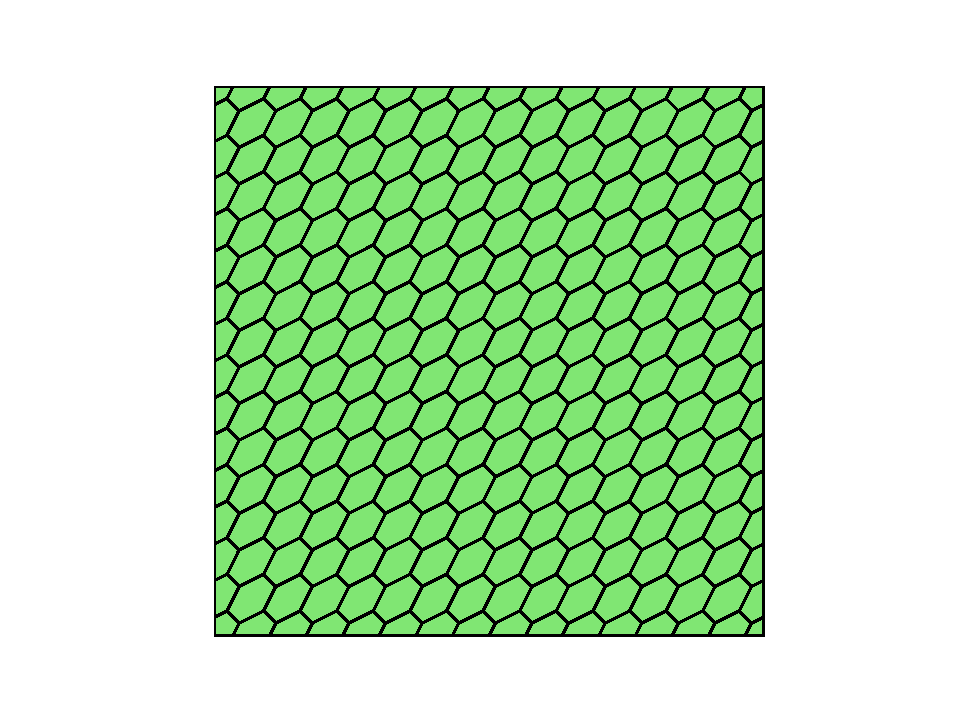
\includegraphics[width=6.0cm]{./figures/stabfree/convex.pdf}
\end{subfigure}%
\hspace{1cm} % 控制子图之间的水平间距
\begin{subfigure}[t]{0.425\linewidth}
    \centering
    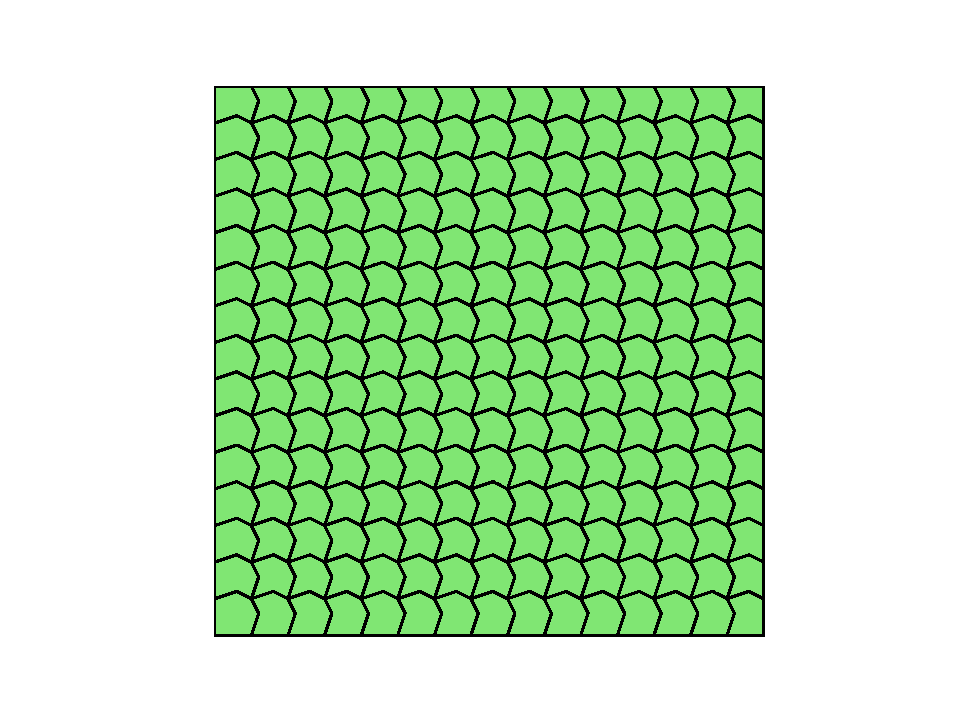
\includegraphics[width=6.0cm]{./figures/stabfree/nonconvex.pdf}
\end{subfigure}
\caption{凸多边形网格(左)和非凸多边形网格(右).}
\label{fig:mesh}
\end{figure}

\subsection{收敛性验证}
\label{sec:convergence}

考虑二阶椭圆问题~\eqref{eq:ellipitc2ndproblem},取 $c = 2$。  
其精确解和源项分别为
\[
    u = \sin(\pi x)\sin(\pi y), \quad f = (2\pi^2+2)\sin(\pi x)\sin(\pi y).
\]

矩形区域 $\Omega$ 分别采用图~\ref{fig:mesh} 所示的凸多边形网格 $\mathcal{T}_0$ 和非凸多边形网格 $\mathcal{T}_1$ 进行离散化。  
在 SFNCVEM 和 SFCVEM 方法中,我们选取 $k = 1, 2, 5$。  
SFNCVEM 在网格 $\mathcal{T}_0$ 和 $\mathcal{T}_1$
上的数值结果如图~\ref{fig:rate1_convex} 和~\ref{fig:rate1_nonconvex} 所示,
可观察到 $\|u - Q_h u_h\|_0 = O(h^{k+1})$,$\|\nabla u - Q_{h, k-1}^{\diver} \nabla_h u_h\|_0 = O(h^{k})$,这与定理~\ref{thm:errorestimateH1} 的理论估计相吻合。  
SFCVEM 的数值结果如图~
\ref{fig:rate2_convex} 和~\ref{fig:rate2_nonconvex} 所示,
同样满足 $\|u - Q_h u_h\|_0 = O(h^{k+1})$,$\|\nabla u - Q_{h, k}^{\diver} \nabla u_h\|_0 = O(h^{k})$,验证了定理~\ref{thm:cfmerrorestimateH1} 的理论收敛率。

\begin{figure}[htp]
\centering
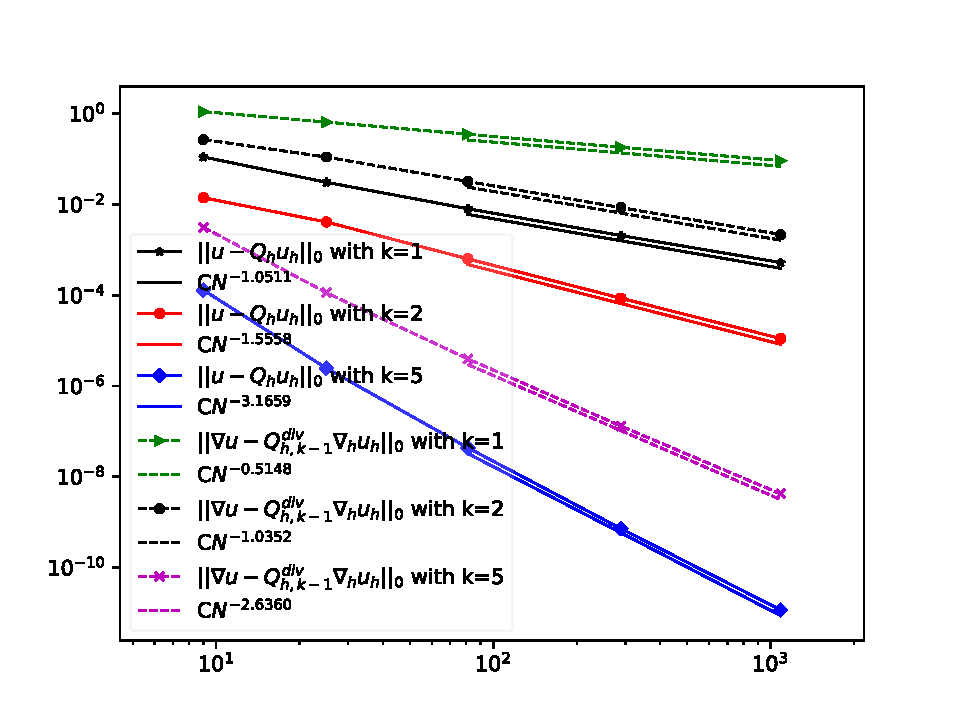
\includegraphics[width=10cm]{./figures/stabfree/ncvem_convex.pdf}
\caption{算例 \ref{sec:convergence} 中非协调虚单元法 \eqref{eq:vem} 在凸网格 $\mathcal T_0$ 上的误差 $\|u - Q_h u_h\|_0$ 和 $\|\nabla u - Q_{h, k-1}^{\diver}\nabla_h u_h\|_0$,其中 $k=1,2,5$。}
\label{fig:rate1_convex}
\end{figure}

\begin{figure}[htp]
\centering
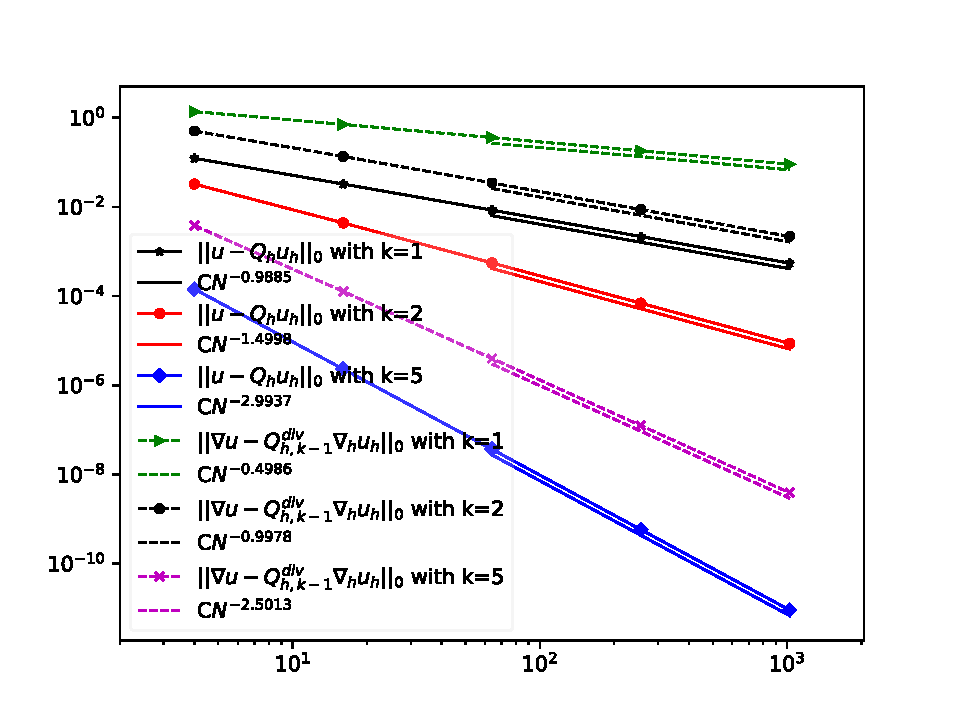
\includegraphics[width=10cm]{./figures/stabfree/ncvem_nonconvex.pdf}
\caption{算例 \ref{sec:convergence} 中非协调虚单元法 \eqref{eq:vem} 在非凸网格 $\mathcal T_1$ 上的误差 $\|u - Q_h u_h\|_0$ 和 $\|\nabla u - Q_{h, k-1}^{\diver}\nabla_h u_h\|_0$,其中 $k=1,2,5$。}
\label{fig:rate1_nonconvex}
\end{figure}


\begin{figure}[htp]
\centering
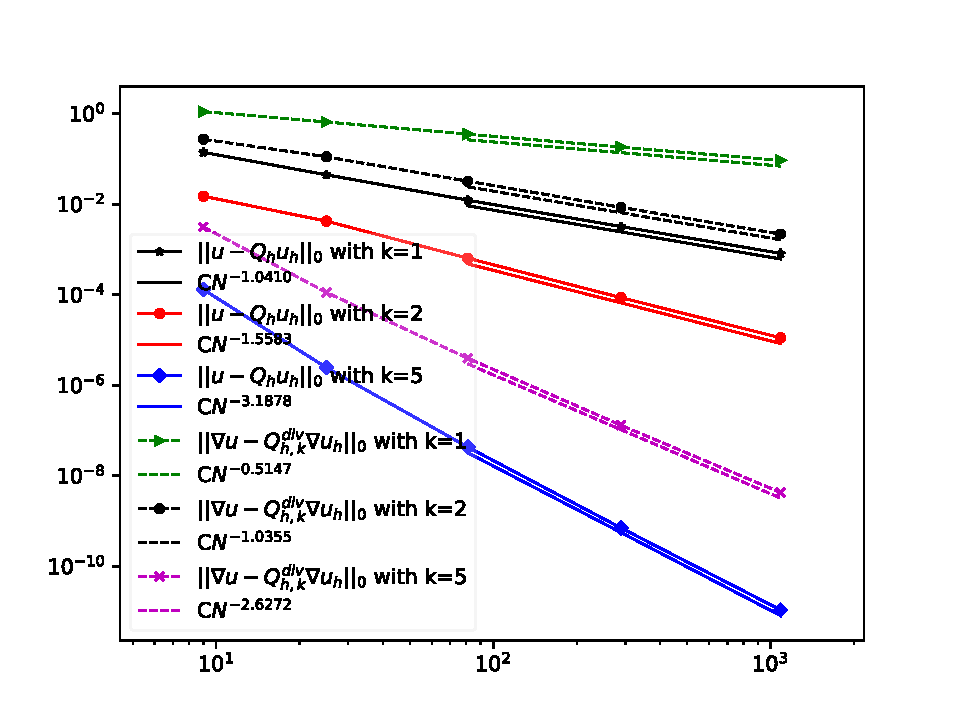
\includegraphics[width=10cm]{./figures/stabfree/cvem_convex.pdf}
\caption{算例 \ref{sec:convergence} 中协调虚单元法 \eqref{eq:cfmvem} 在凸网格 $\mathcal T_0$ 上的误差 $\|u - Q_h u_h\|_0$ 和 $\|\nabla u - Q_{h, k}^{\diver}\nabla u_h\|_0$,其中 $k=1,2,5$。}
\label{fig:rate2_convex}
\end{figure}

\begin{figure}[htp]
\centering
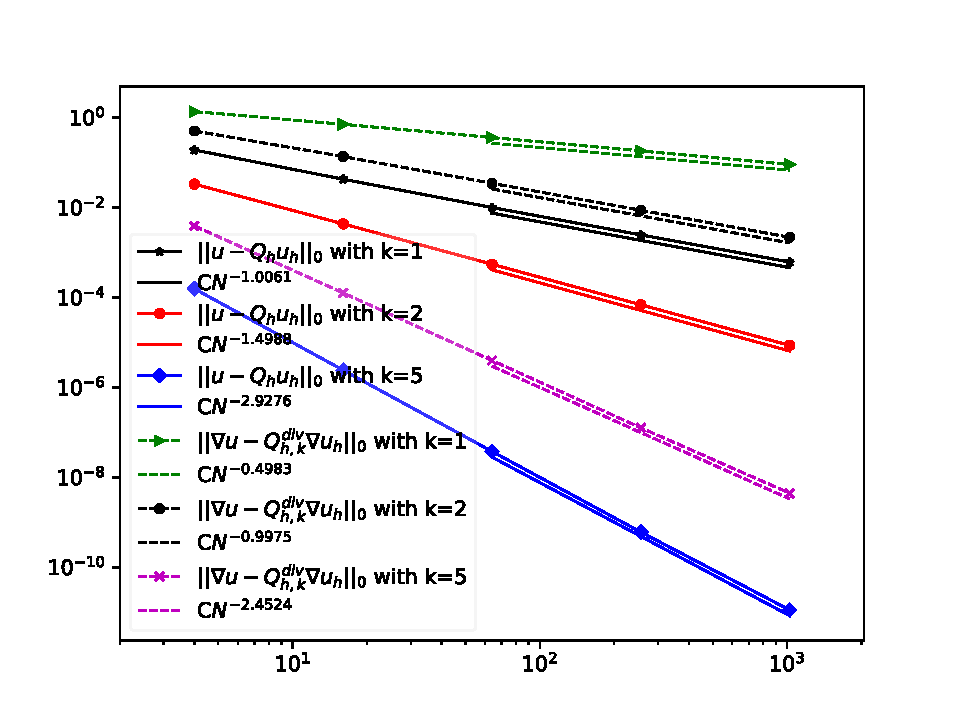
\includegraphics[width=10cm]{./figures/stabfree/cvem_nonconvex.pdf}
\caption{算例 \ref{sec:convergence} 中协调虚单元法 \eqref{eq:cfmvem} 在非凸网格 $\mathcal T_1$ 上的误差 $\|u - Q_h u_h\|_0$ 和 $\|\nabla u - Q_{h, k}^{\diver}\nabla u_h\|_0$,其中 $k=1,2,5$。}
\label{fig:rate2_nonconvex}
\end{figure}


\subsection{局部刚度矩阵的可逆性}
\label{sec:stability}
我们构造了图 \ref{fig:hexagon} 所示的三种不同六边形,并计算了 $k=3$
时四种虚单元方法的局部刚度矩阵的特征值。数值结果表明,在三种六边形上,SFNCVEM
和 SFCVEM 都仅有一个零特征值。此外,在表
\ref{tab:comparison0}-\ref{tab:comparison2}
中,我们展示了不同六边形上的局部刚度矩阵的最小非零特征值、最大特征值和条件数。
可以看出,这些数值在四种虚单元方法之间是基本相同的。

\begin{figure}[htbp]
\centering
\begin{subfigure}[t]{0.3\linewidth}
    \centering
    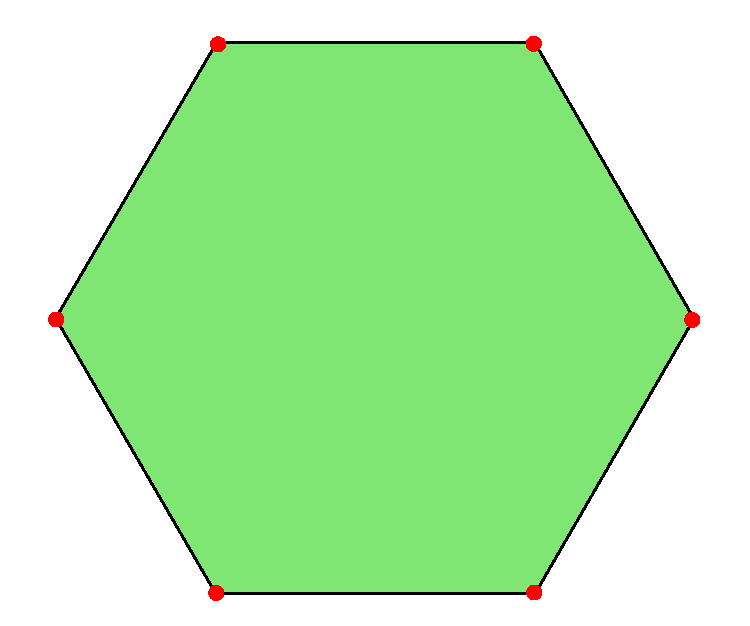
\includegraphics[width=1in]{./figures/stabfree/hexagon0.pdf}
    \caption{正六边形}
    \label{fig:hexagon0}
\end{subfigure}%
\hspace{0.5cm} % 控制子图之间的水平间距
\begin{subfigure}[t]{0.3\linewidth}
    \centering
    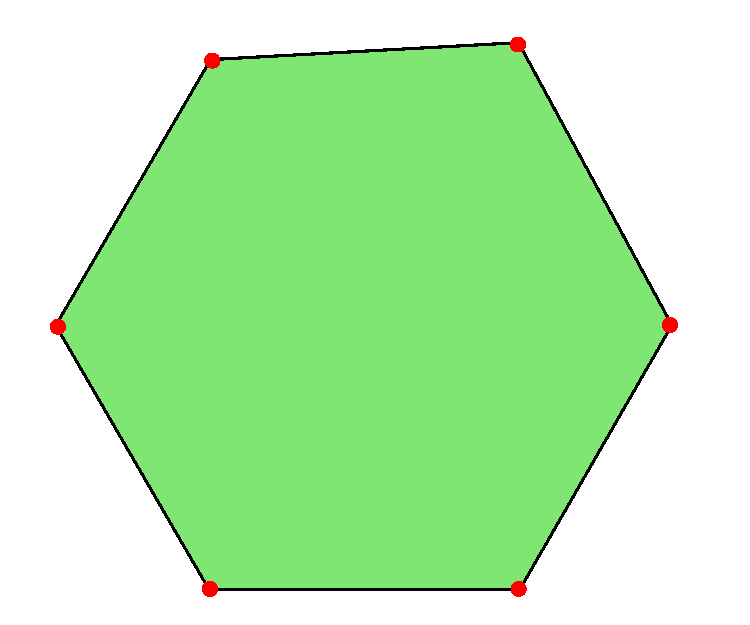
\includegraphics[width=1in]{./figures/stabfree/hexagon1.pdf}
    \caption{由正六边形微小扰动生成的拟正六边形}
    \label{fig:hexagon1}
\end{subfigure}%
\hspace{0.5cm} % 控制子图之间的水平间距
\begin{subfigure}[t]{0.3\linewidth}
    \centering
    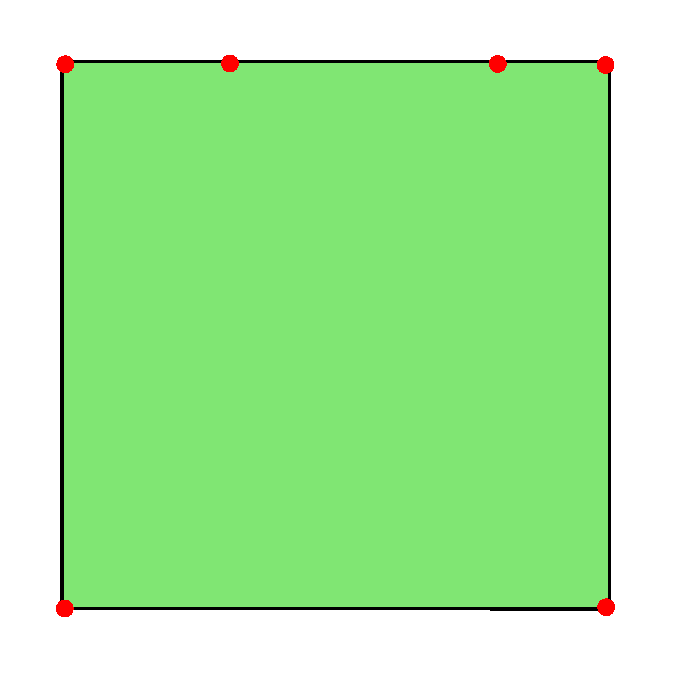
\includegraphics[width=0.9in]{./figures/stabfree/hexagon2.pdf}
    \caption{具有两个悬点的正方形}
    \label{fig:hexagon2}
\end{subfigure}
\caption{正六边形(左)、由正六边形微小扰动生成的拟正六边形(中)、以及具有两个悬点的正方形(右).}
\label{fig:hexagon}
\end{figure}


\begin{table}[htbp]
\centering
\caption{算例 \ref{sec:stability} 中,
正六边形上特征值及条件数的比较.}
\label{tab:comparison0}
\begin{tabular}{c|c c c}
\hline
\textbf{方法} & \textbf{最大特征值} & \textbf{最小非零特征值} & \textbf{条件数} \\\hline
NCVEM  & 975.5693189 & 0.309674737 & 3150.303211 \\\hline
CVEM   & 1012.488116 & 0.297206358 & 3406.683909 \\\hline
SFNCVEM & 992.5956147 & 0.318932029 & 3112.248147 \\\hline
SFCVEM  & 1011.173331 & 0.298509692 & 3387.405362 \\\hline
\end{tabular}
\end{table} 

\begin{table}[htbp]
\centering
\caption{算例 \ref{sec:stability} 中,
拟正六边形上特征值及条件数的比较.}
\label{tab:comparison1}
\begin{tabular}{c|c c c}
\hline
\textbf{方法} & \textbf{最大特征值} & \textbf{最小非零特征值} & \textbf{条件数} \\\hline
NCVEM  & 935.2883848 & 0.279027715 & 3351.955143 \\\hline
CVEM   & 1014.672395 & 0.257370621 & 3942.456177 \\\hline
SFNCVEM & 997.4831245 & 0.282126359 & 3535.589964 \\\hline
SFCVEM  & 1047.876056 & 0.258970708 & 4046.311124 \\\hline
\end{tabular}
\end{table}

\begin{table}[htbp]
\centering
\caption{算例 \ref{sec:stability} 中,
带有两个悬点的正方形上特征值及条件数的比较.}
\label{tab:comparison2}
\begin{tabular}{c|c c c}
\hline
\textbf{方法} & \textbf{最大特征值} & \textbf{最小非零特征值} & \textbf{条件数} \\\hline
NCVEM  & 941.8571938 & 0.21069027 & 4470.340249 \\\hline
CVEM   & 1046.755495 & 0.200435123 & 5222.4155 \\\hline
SFNCVEM & 986.5963357 & 0.212761106 & 4637.108513 \\\hline
SFCVEM  & 1061.651989 & 0.202074633 & 5253.761808 \\\hline
\end{tabular}
\end{table}

\subsection{刚度矩阵组装时间的比较}
\label{sec:stiffnessmatrixassembly}
标准虚单元方法和无稳定化项的虚单元方法之间唯一的区别是刚度矩阵,
因此我们通过分别改变多项式次数$k$和网格尺寸$h$来详细比较四种不同方法 
在组装刚度矩阵时所消耗的时间。我们在本实验中使用图~\ref{fig:mesh}(a)中的网格。
表~\ref{tab:ptime}和表~\ref{tab:ttime}中的结果显示,NCVEM、CVEM和SFNCVEM的组装时间相似。
然而,由于需要将投影映射到更高次的多项式空间,SFCVEM的计算时间较长。

\begin{table}[H]
    \caption{算例 \ref{sec:stiffnessmatrixassembly} 中,
    在$h=0.2$和不同$k$下,四种虚单元方法组装刚度矩阵所消耗的时间.}
\label{tab:ptime}
\centering
\begin{tabular}{c|cccc}
\hline
$k$ & 2 & 4 & 8 & 10 \\
\hline
SFCVEM & 0.053684235 & 0.144996881 & 1.468627453 & 2.603836536 \\
SFNCVEM & 0.022516727 & 0.065697193 & 0.806378841 & 1.554260015 \\
CVEM & 0.021185875 & 0.059809923 & 0.600241184 & 1.160929918 \\
NCVEM & 0.0213027 & 0.061014891 & 0.596506596 & 1.129639149 \\
\hline
\end{tabular}
\end{table}

\begin{table}[H]
    \caption{算例 \ref{sec:stiffnessmatrixassembly} 中,
    在$k = 5$和不同$h$下,四种虚单元方法组装刚度矩阵所消耗的时间.}
\label{tab:ttime}
\centering
\begin{tabular}{c|cccc}
\hline
$h$ & 1 & 0.25 & 0.0625 & 0.03125 \\
\hline
SFCVEM & 0.039689541 & 0.199015379 & 1.74412179 & 4.75462532 \\
SFNCVEM & 0.018287182 & 0.100006819 & 0.81251812 & 2.465409517 \\
CVEM & 0.018686771 & 0.087426662 & 0.781031132 & 1.983617783 \\
NCVEM & 0.018309593 & 0.096345425 & 0.767129898 & 2.159288645 \\
\hline
\end{tabular}
\end{table}

\begin{figure}[H]
\centering
\begin{subfigure}[t]{0.3\linewidth}
    \centering
    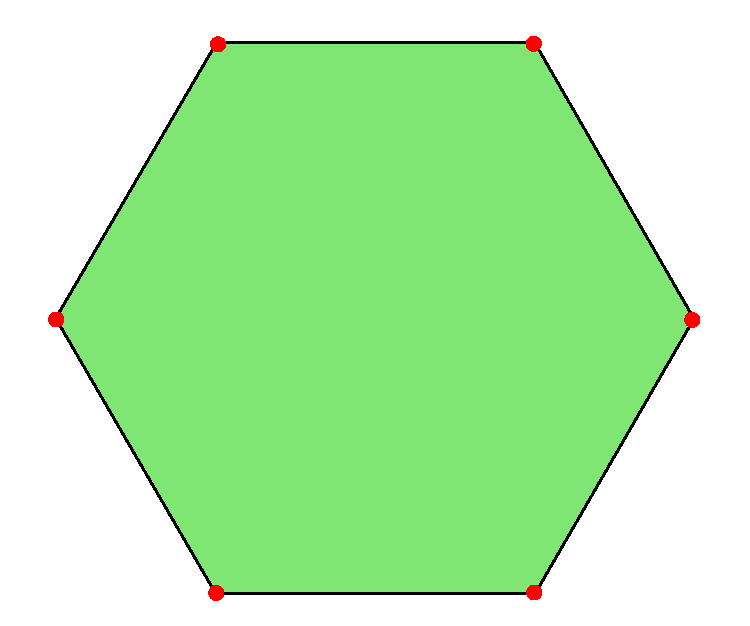
\includegraphics[width=1in]{./figures/stabfree/hexagon0.pdf}
\end{subfigure}%
\hspace{0.5cm}
\begin{subfigure}[t]{0.3\linewidth}
    \centering
    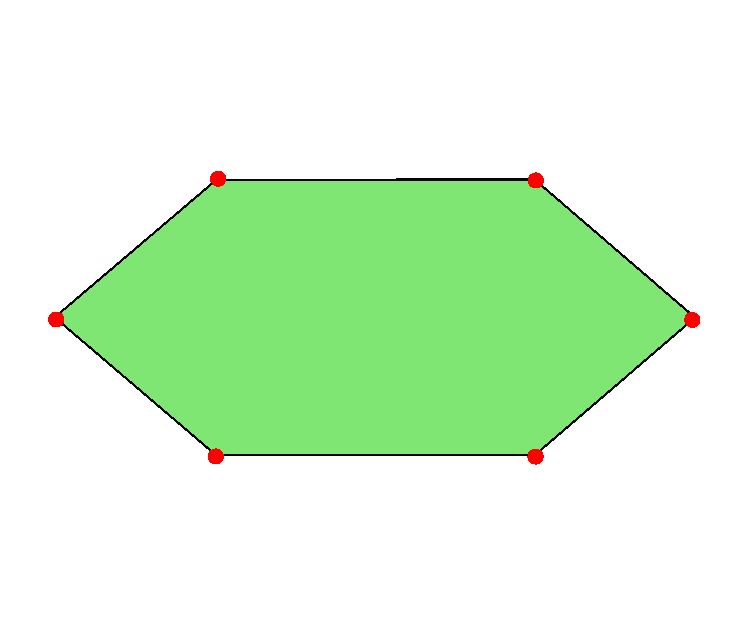
\includegraphics[width=1in]{./figures/stabfree/hexagon3.pdf}
\end{subfigure}%
\hspace{0.5cm}
\begin{subfigure}[t]{0.3\linewidth}
    \centering
    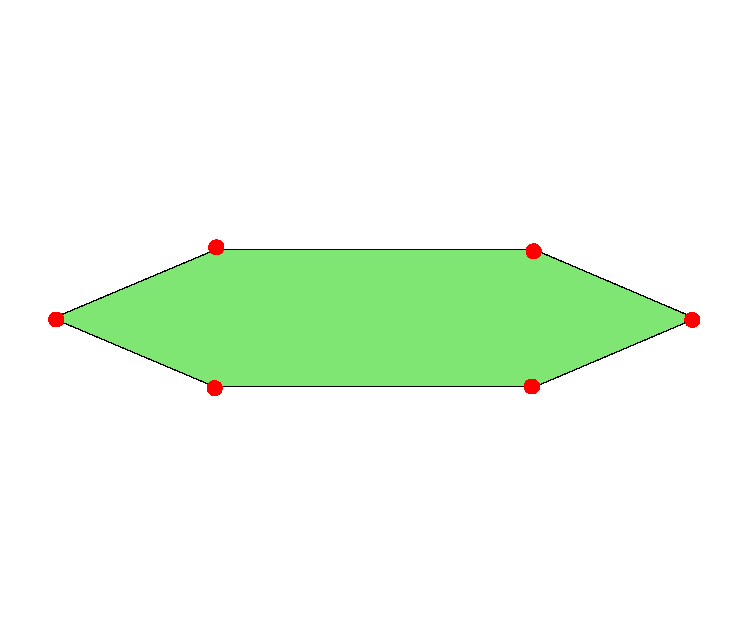
\includegraphics[width=1in]{./figures/stabfree/hexagon4.pdf}
\end{subfigure}
\caption{六边形 $H_0, H_1, H_2$.}
\label{fig:collapsehexagon}
\end{figure}

\subsection{刚度矩阵的条件数}
\label{sec:conditionnumber}
我们设计了两个实验来检查四种虚单元方法刚度矩阵的条件数。

首先,我们参考文献 \cite{Mascotto2018} 中的 “收缩多边形” 实验,
考虑一个六边形序列 $\{H_i\}_{i=0}^{\infty}$,其中 $H_i$ 
的顶点分别为 $A_i = (1, 0)$,$B_i = (0.5, a_i)$,$C_i = (-0.5, a)$,$D_i = (-1,
0)$,$E_i = (-0.5, -a_i)$ 和 $F_i = (0.5, -a_i)$,其中 $a_i =
\frac{\sqrt{3}}{2^{i+1}}$。图 \ref{fig:collapsehexagon} 展示了六边形
$H_0$,$H_1$ 和 $H_2$。

如图 \ref{fig:collapsehexagon_conditionnumber} 所示,对于 $k=8$ 和 $k=10$,当
$i$ 较大时,无稳定化项的虚单元方法刚度矩阵的条件数比标准方法要小。

\begin{figure}[htbp]
\centering
\begin{subfigure}[t]{0.45\linewidth}
\centering
\includegraphics*[width=3in]{./figures/stabfree/collapsing_condition_number_8.pdf}
\caption{$k = 8$}
\end{subfigure}%%
\quad \quad
\begin{subfigure}[t]{0.45\linewidth}
\centering
\includegraphics*[width=3in]{./figures/stabfree/collapsing_condition_number_10.pdf}
\caption{$k = 10$}
\end{subfigure}
\caption{算例 \ref{sec:conditionnumber} 中,
四种虚单元方法在 $\{H_i\}_{i=0}^{12}$ 上的刚度矩阵条件数.}
\label{fig:collapsehexagon_conditionnumber}
\end{figure}

其次,我们对二阶椭圆方程进行 Patch Test,
即求解问题 \eqref{eq:ellipitc2ndproblem},其中 $c =
0$,$f=0$,但狄利克雷边界条件为非齐次,取精确解 $u = 1+x+y$。
我们考虑以下三种情况下四种虚单元方法的误差 $\|u - u_h\|_0$:
\begin{enumerate}[(1)]
\item 图 \ref{fig:mesh}(a) 中的网格:固定 $h_x = h_y = 0.2$,但 $k=1, 2, \ldots, 10$;
\item 图 \ref{fig:mesh}(a) 中的网格:固定 $k=3$,但变化 $h_x = h_y = 2^{-i}$,其中 $i=1, \ldots, 5$;
\item 图 \ref{fig:polymeshhy} 中的网格:固定 $k=3$ 和 $h_x=0.2$,但变化 $h_y = 2^{-i}$,其中 $i=1, \ldots, 8$。
\end{enumerate}

\begin{figure}[htp]
\centering
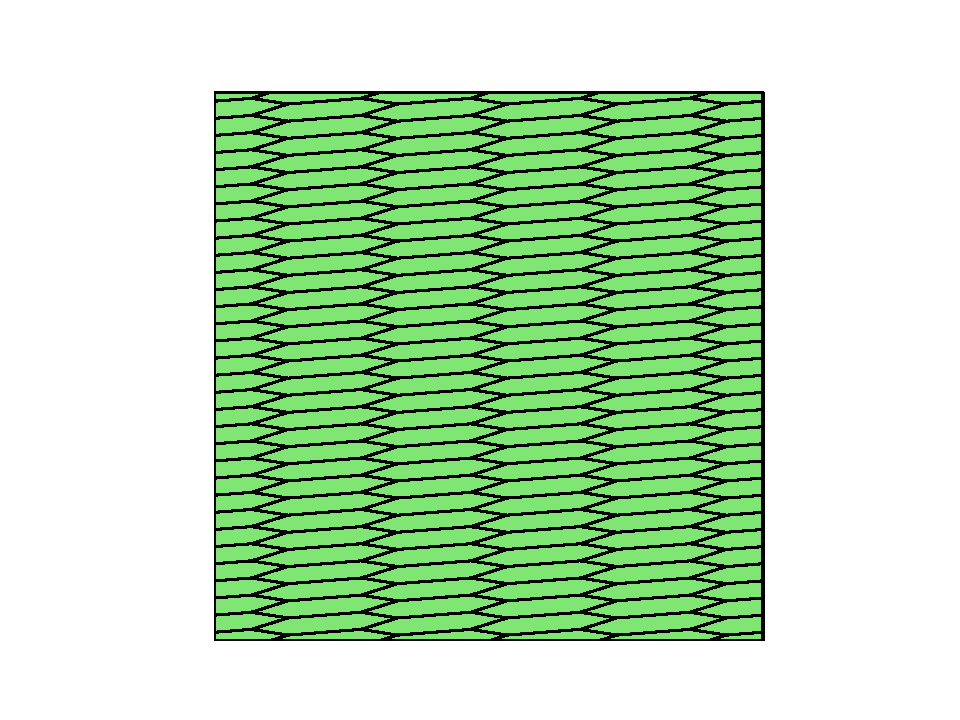
\includegraphics[width=3in]{./figures/stabfree/mesh_hy.pdf}
\caption{算例 \ref{sec:conditionnumber} 中,
网格在区域 $(0, 1) \times (0, 1)$ 上,$h_x = 0.2$,$h_y = 0.03125$.}
\label{fig:polymeshhy}
\end{figure}

如图 \ref{fig:patchtest_p}, 
所示,四种方法的误差相似。
因为刚度矩阵条件数的增大,Patch Test 的误差也随之增大,
四种方法得到的刚度矩阵条件数是相似的。
\begin{figure}[htp]
\centering
\begin{subfigure}[t]{0.45\linewidth}
\centering
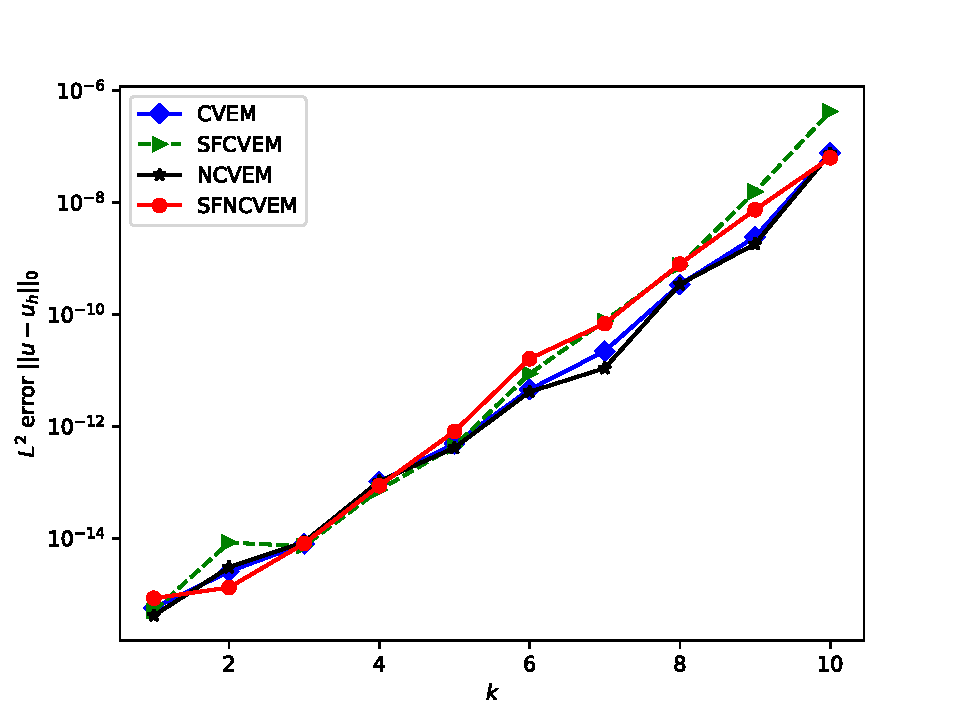
\includegraphics[width=3.0in]{./figures/stabfree/patch_test_p.pdf}
\end{subfigure}%%
\begin{subfigure}[t]{0.45\linewidth}
\centering
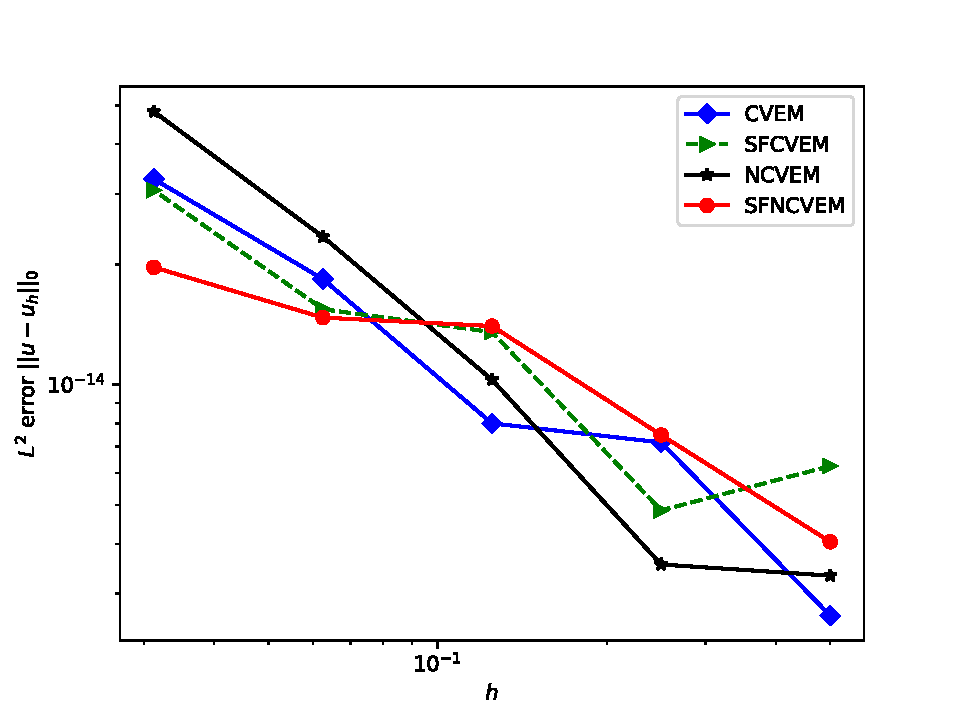
\includegraphics[width=3.0in]{./figures/stabfree/patch_test_h.pdf}
\end{subfigure}
\caption{算例 \ref{sec:conditionnumber} 中,固定 $h_x, h_y$(左)和固定
$k$(右)时,四种虚单元方法的 Patch Test 的 $L^2$ 误差.}
\label{fig:patchtest_ph}
\end{figure}


\begin{figure}[htp]
\centering
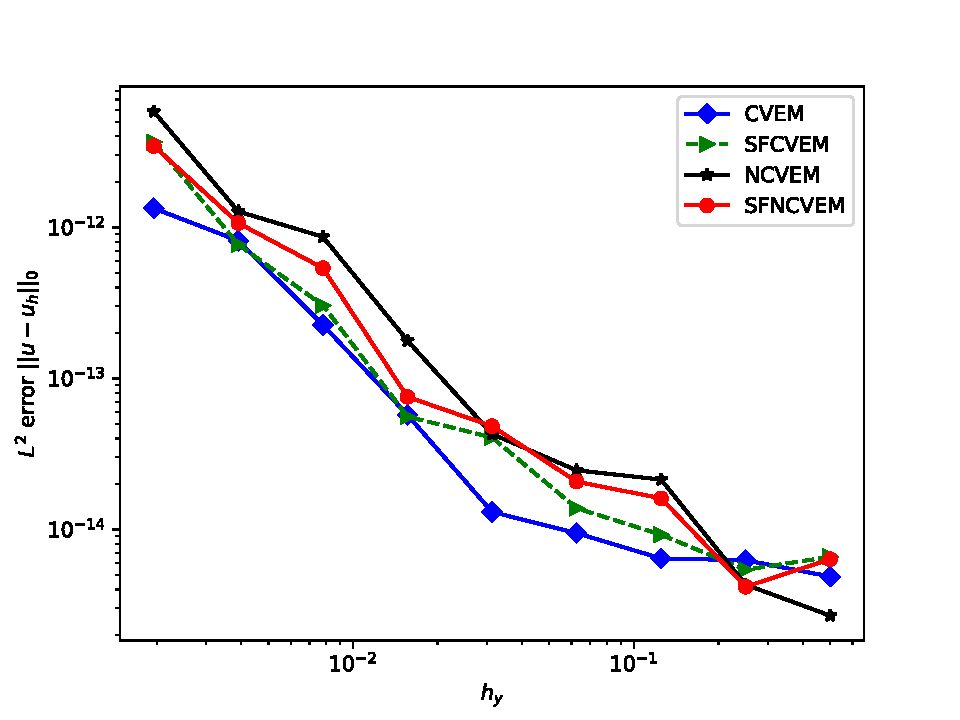
\includegraphics[width=3.2in]{./figures/stabfree/patch_test_hy.pdf}
\caption{算例 \ref{sec:conditionnumber} 中,固定 $k, h_x$ 但变化 $h_y$ 时,
四种虚单元方法的 Patch Test 的 $L^2$ 误差.}
\label{fig:patchtest_hy}
\end{figure}


